\documentclass[conference]{IEEEtran}
\IEEEoverridecommandlockouts
% The preceding line is only needed to identify funding in the first footnote. If that is unneeded, please comment it out.
\usepackage[utf8]{inputenc}
\usepackage[vietnamese]{babel}
\usepackage{amsmath}
\usepackage{cite}
\usepackage{amsmath,amssymb,amsfonts}
\usepackage{algorithmic}
\usepackage{graphicx}
\usepackage{textcomp} 
\usepackage{xcolor}
\usepackage{biblatex}
\addbibresource{ref.bib}
\usepackage{fancyhdr}
\usepackage{adjustbox}
\usepackage{lipsum}

\pagestyle{fancy}
\fancyhf{}
\rfoot{\thepage}
\def\BibTeX{{\rm B\kern-.05em{\sc i\kern-.025em b}\kern-.08em
    T\kern-.1667em\lower.7ex\hbox{E}\kern-.125emX}}
\begin{document}

\title{ỨNG DỤNG CÁC MÔ HÌNH THỐNG KÊ, MÁY HỌC VÀ HỌC SÂU ĐỂ DỰ BÁO GIÁ KIM LOẠI QUÝ\\
}

\author{\IEEEauthorblockN{1. Phan Minh Trí}
\IEEEauthorblockA{\textit{Khoa Hệ thống Thông tin} \\
\textit{Trường Đại học Công nghệ Thông tin}\\
21522709@gm.uit.edu.vn}
\and
\IEEEauthorblockN{2. Vương Thanh Linh}
\IEEEauthorblockA{\textit{Khoa Hệ thống Thông tin} \\
\textit{Trường Đại học Công nghệ Thông tin}\\
21521082@gm.uit.edu.vn}
\and
\IEEEauthorblockN{3. Lê Nguyễn Hoàng Huy}
\IEEEauthorblockA{\textit{Khoa Hệ thống Thông tin} \\
\textit{Trường Đại học Công nghệ Thông tin}\\
21520915@gm.uit.edu.vn}
\and
\IEEEauthorblockN{4. Trần Hạnh Thảo}
\IEEEauthorblockA{\textit{Khoa Hệ thống Thông tin} \\
\textit{Trường Đại học Công nghệ Thông tin}\\
21522609@gm.uit.edu.vn}
\and
\IEEEauthorblockN{                }
\IEEEauthorblockA{\textit{                      } \\
\textit{                                  }\\
                     }
                     \and
\IEEEauthorblockN{                }
\IEEEauthorblockA{\textit{                      } \\
\textit{                                  }\\
                     }
                     \and
\IEEEauthorblockN{                }
\IEEEauthorblockA{\textit{                      } \\
\textit{                                  }\\
                     }
                     \and
\IEEEauthorblockN{                }
\IEEEauthorblockA{\textit{                      } \\
\textit{                                  }\\
                     }
                     \and
\IEEEauthorblockN{                }
\IEEEauthorblockA{\textit{                      } \\
\textit{                                  }\\
                     }
                     \and
\IEEEauthorblockN{                }
\IEEEauthorblockA{\textit{                      } \\
\textit{                                  }\\
                     }\and
\IEEEauthorblockN{                }
\IEEEauthorblockA{\textit{                      } \\
\textit{                                  }\\
                     }
\and
\IEEEauthorblockN{5. Nguyễn Thị Tường Vi}
\IEEEauthorblockA{\textit{Khoa Hệ thống Thông tin} \\
\textit{Trường Đại học Công nghệ Thông tin}\\
21522787@gm.uit.edu.vn}
}

\maketitle
\thispagestyle{fancy}
\begin{abstract}
Trên thị trường hiện nay, vàng (gold), bạch kim (platinum) và palladium là các kim loại quý hiếm, có giá trị cao và nhu cầu về các kim loại này không bao giờ lỗi thời. Xu hướng tỷ giá của kim loại quý cho thấy vàng, bạch kim và palladium là một trong những phương án đầu tư tốt nhất hiện nay. Vì vậy, để hiểu rõ và dự đoán xu hướng của tỷ giá này có ý nghĩa như thế nào đối với nền kinh tế đất nước. Bài báo sẽ nghiên cứu các ý tưởng dự đoán tỷ giá vàng (gold), bạch kim (platinum) và palladium bằng các mô hình dự báo: AMIRA, RNN, GRU, LSTM, ETS, LN, SVM, Random Forest, TimesNet, Autoformer. Nghiên cứu áp dụng 10 mô hình dự báo khác nhau để tìm ra mô hình nào hoạt động tốt nhất trên tập dữ liệu có sẵn và mang lại kết quả tốt nhất cho việc đầu tư.
\end{abstract}

Từ khóa: Phân tích chuỗi thời gian, dự báo, LR, ETS, AMIRA, RF, SVM, RNN, GRU, LSTM, TimesNet, Autoformer

\section{ĐẶT VẤN ĐỀ}
Hiện tại, trong bối cảnh nền kinh tế thế giới nói chung và Việt Nam nói riêng đang diễn biến 1 cách phức tạp và khó dự đoán kể từ sau đại dịch COVID-19. Các lĩnh vực chủ đạo của nền kinh tế ít nhiều bị biến động, do đó giá của các kim loại quý như vàng (Gold), bạch kim (Platinum) và Palladium cũng bị biến động theo nền kinh tế hiện tại. Và việc dự báo giá cũng là 1 vấn đề quan trọng trong lĩnh vực tài chính và đầu tư. Việc dự báo chính xác giá của các kim loại quý này có thể giúp các nhà đầu tư, doanh nghiệp và các tổ chức khác đưa ra quyết định sáng suốt về việc mua bán, nắm giữ hoặc đầu tư vào chúng. Nắm bắt được vấn đề hiện hữu, nhóm chúng tôi đã thực hiện nghiên cứu này với các mô hình dự báo chuỗi thời gian để có thể đưa ra được các dự báo với tỉ lệ chính xác cao nhằm giúp ích cho việc phát triển và đầu tư.

Để dự báo giá của các kim loại quý, có khá nhiều thuật toán và kỹ thuật hỗ trợ cho việc này. Và trong nghiên cứu này, chúng tôi sẽ sử dụng 10 mô hình để áp dụng cho việc dự báo bao gồm: Linear Regression (LR), Exponential Smoothing Trend (ETS), ARIMA, Random Forest (RF), Support Vector Regression (SVR), Recurrent Neural Network (RNN), Gated Recurrent Unit  (GRU), Long Short Term Memory (LSTM), Timesnet, Autoformer. Những mô hình này được áp dụng và sẽ dự báo giá của kim loại quý trong 30, 60 và 90 ngày tới.

Dựa vào kết quả dự báo, chúng tôi có thể phân tích, đánh giá và kiểm tra độ chính xác của các giá dự báo bằng cách so sánh với giá thực tế. Điều này giúp tinh chỉnh các mô hình và phương pháp dự báo để đạt độ chính xác cao hơn. Ngoài ra, các kết quả dự báo này có thể sẽ giúp cho các nhà đầu tư, doanh nghiệp và các tổ chức tài chính để họ sử dụng trong việc lập kế hoạch và quyết định đầu tư.

\section{CƠ SỞ LÝ THUYẾT}
Dự báo giá vàng bằng ARIMA, RW, ARFIMA, ETS, TBATS và MLR. Nghiên cứu của Alessio Azzutti\cite{azzu} , so sánh kết quả thu được từ 6 mô hình dự báo, để dự báo giá vàng. Nghiên cứu gồm 36 phạm vi dự báo khác nhau cả về dài hạn và ngắn hạn, từ kết quả thu được ta nhận thấy không có mô hình nào trong 6 mô hình có thể đưa ra dự báo chính xác nhất về giá vàng trong cả ngắn hạn và dài hạn. Tuy nhiên dựa trên RMSE thì ARIMA cung cấp dự báo tốt hơn lần lượt là 5\%, 2\%, 1\%, 54\% và 55\% so với mô hình RW, ETS, TBATS, ARFIMA và MLR.

\begin{figure}[htbp]
\centerline{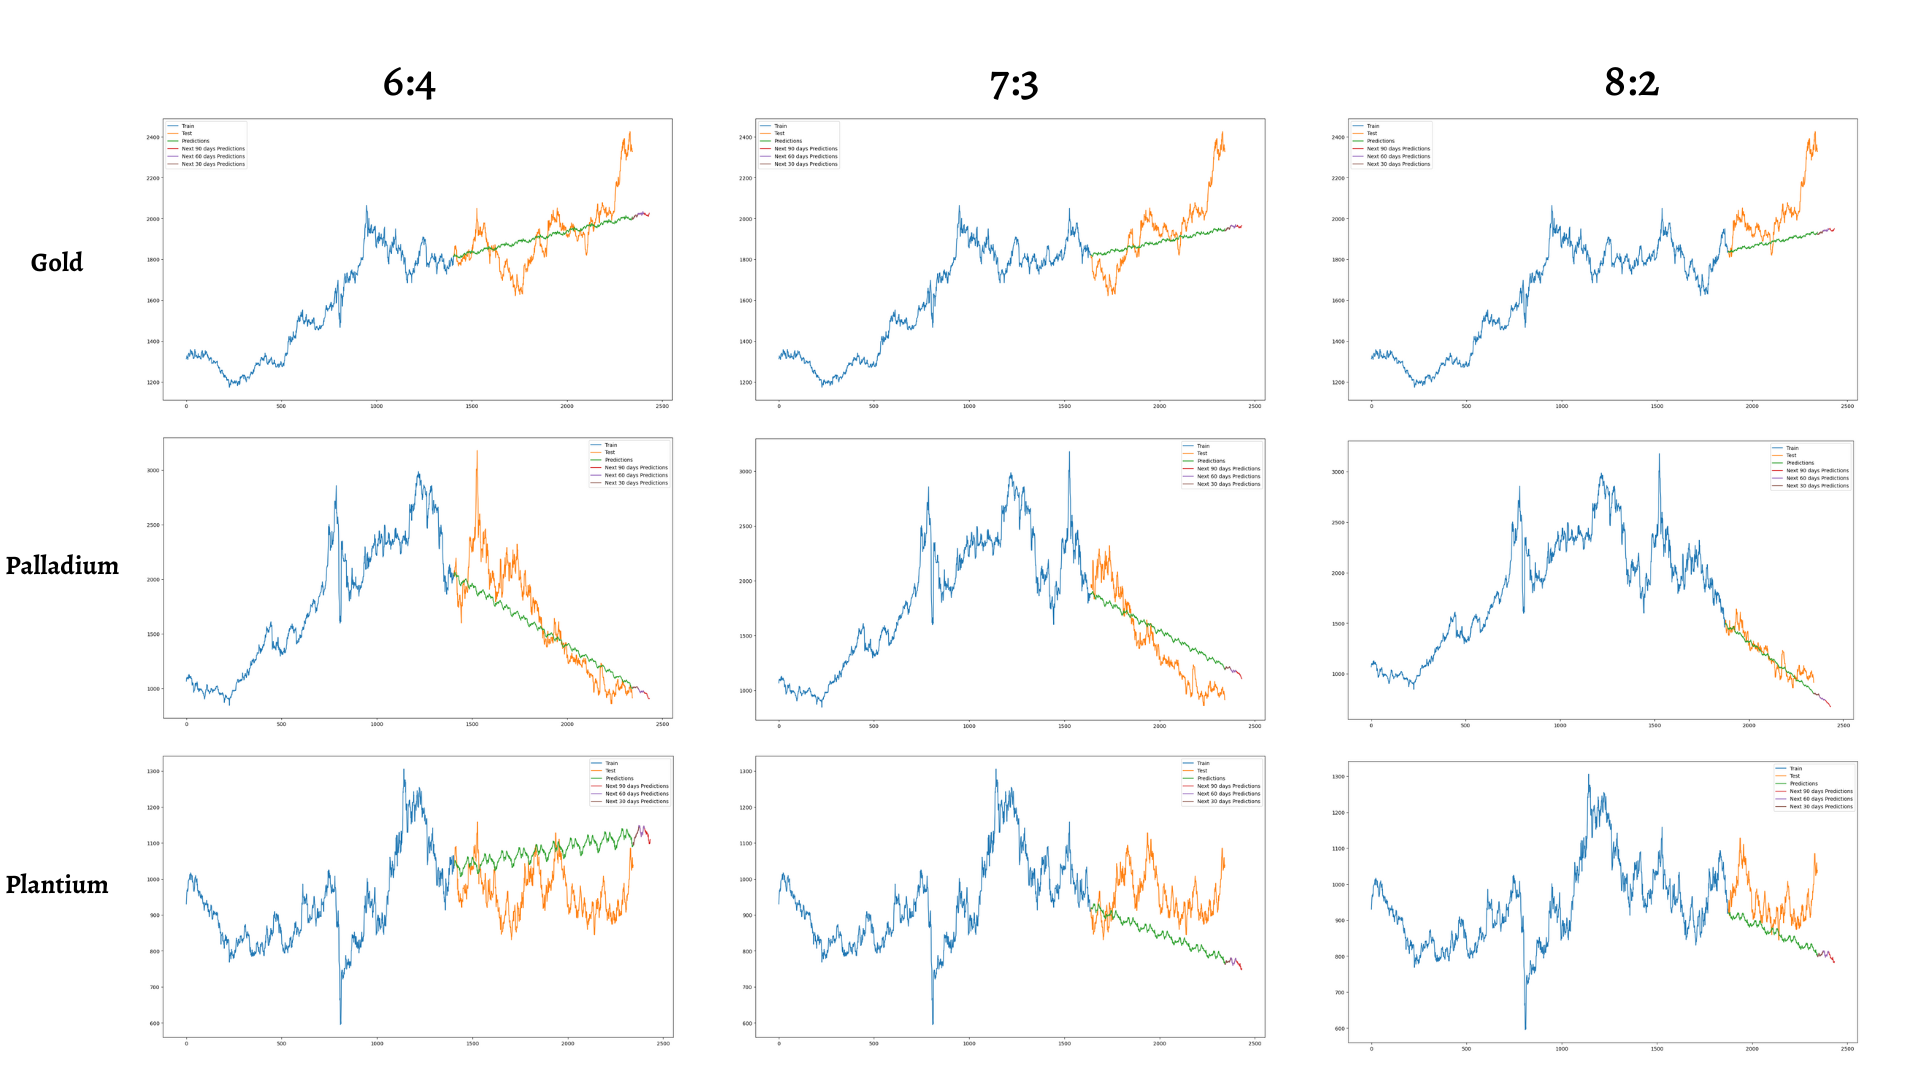
\includegraphics[width=0.5\textwidth]{img/ETS_result.png}}
\caption{Kết quả thực nghiệm ETS}
\label{fig}
\end{figure}

Dự đoán giá vàng sử dụng mô hình ARIMA được nghiên cứu bởi Banhi Guha và Gautam Bandyopadhyay\cite{article2}. Trong nghiên cứu này, họ đã phân tích hiệu suất giá vàng trong 10 năm qua. Dựa trên giá được giao dịch trên MCX, trong sáu bộ tham số mô hình khác nhau cho thấy ARIMA(1,1,1) là mô hình dự đoán tốt nhất cho các giá trị tương lai của vàng và đáp ứng được tất cả các tiêu chí thống kê phù hợp.

\begin{figure}[H]
\centerline{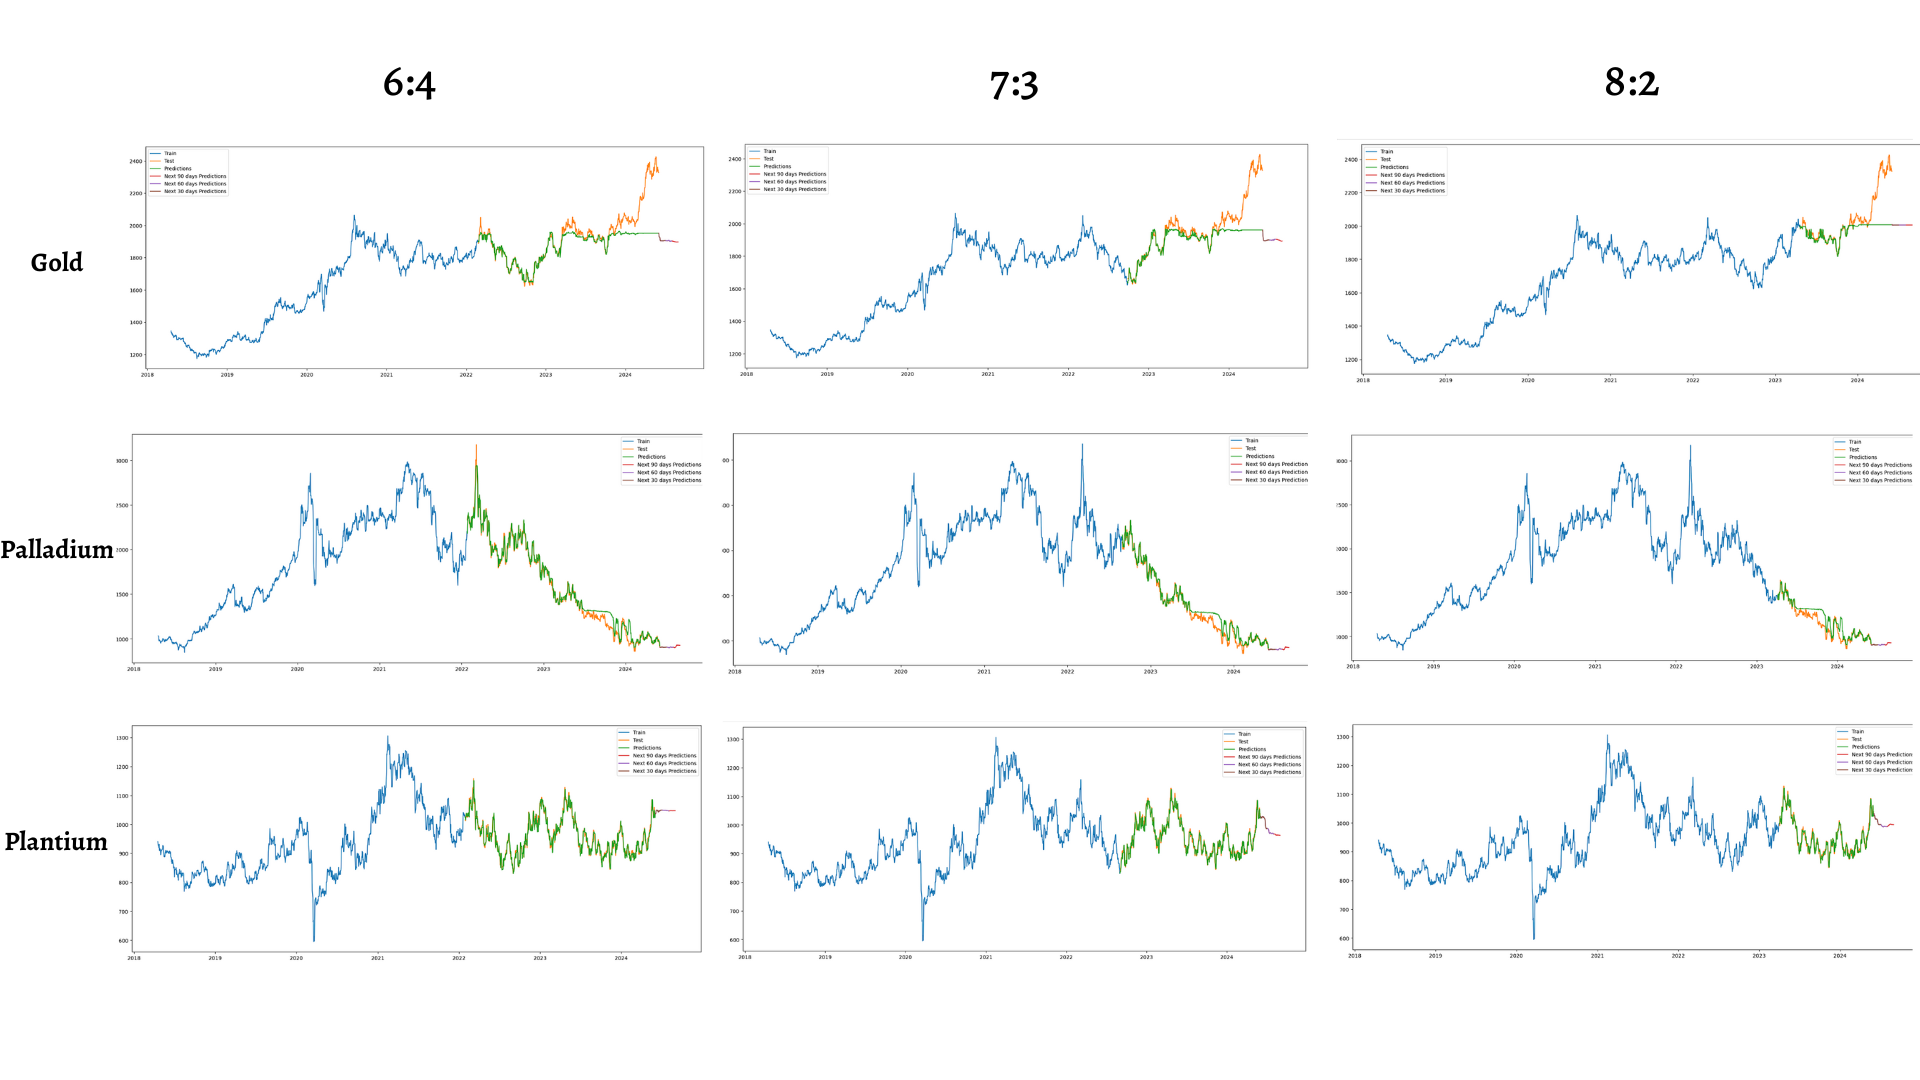
\includegraphics[width=0.45\textwidth]{img/RF_result.png}}
\caption{Kết quả thực nghiệm Random Forest}
\label{fig}
\end{figure}

\begin{figure}[H]
\centerline{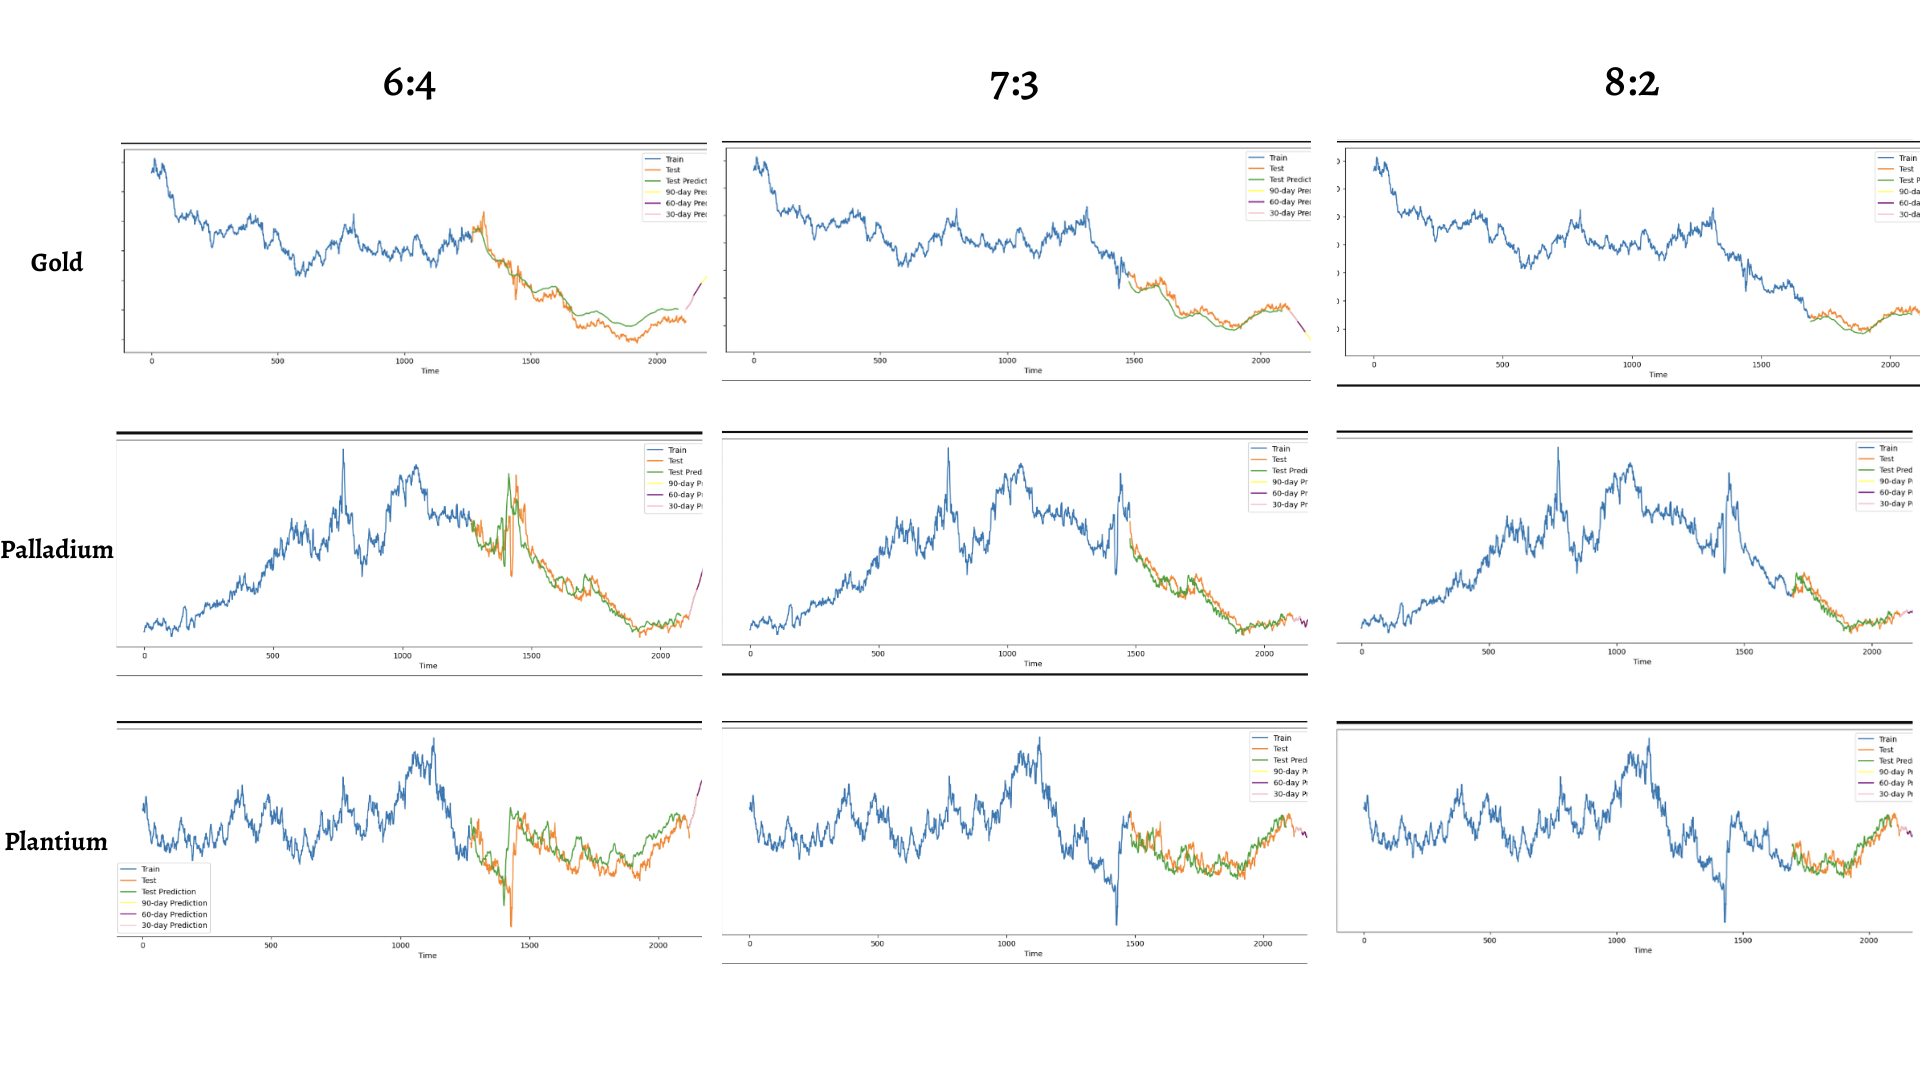
\includegraphics[width=0.45\textwidth]{img/SVR_result.png}}
\caption{Kết quả thực nghiệm SVR}
\label{fig}
\end{figure}

Madini O. Alassafi, Mutasem Jarrah, Reem Alotaibi\cite{10263962} đã sử dụng mô hình RNN và LSTM  để dự đoán sự lây lan của COVID-19 ở Malaysia, Morocco và Ả Rập Xê Út. Nghiên cứu cũng so sánh số ca mắc bệnh và số ca tử vong do COVID-19 ở Malaysia, Morocco và Ả Rập Xê Út. Sau đó, họ dự đoán số ca mắc và tử vong trong 7 ngày tiếp theo dựa trên dữ liệu có sẵn đến ngày 3 tháng 12 năm 2020. Kết quả độ chính xác của các mô hình lần lượt là 97.34\% RNN (Sigmoid), 93.32\% RNN (Tanh) và 99.27\% LSTM (ReLU). 

\begin{figure}[htbp]
\centerline{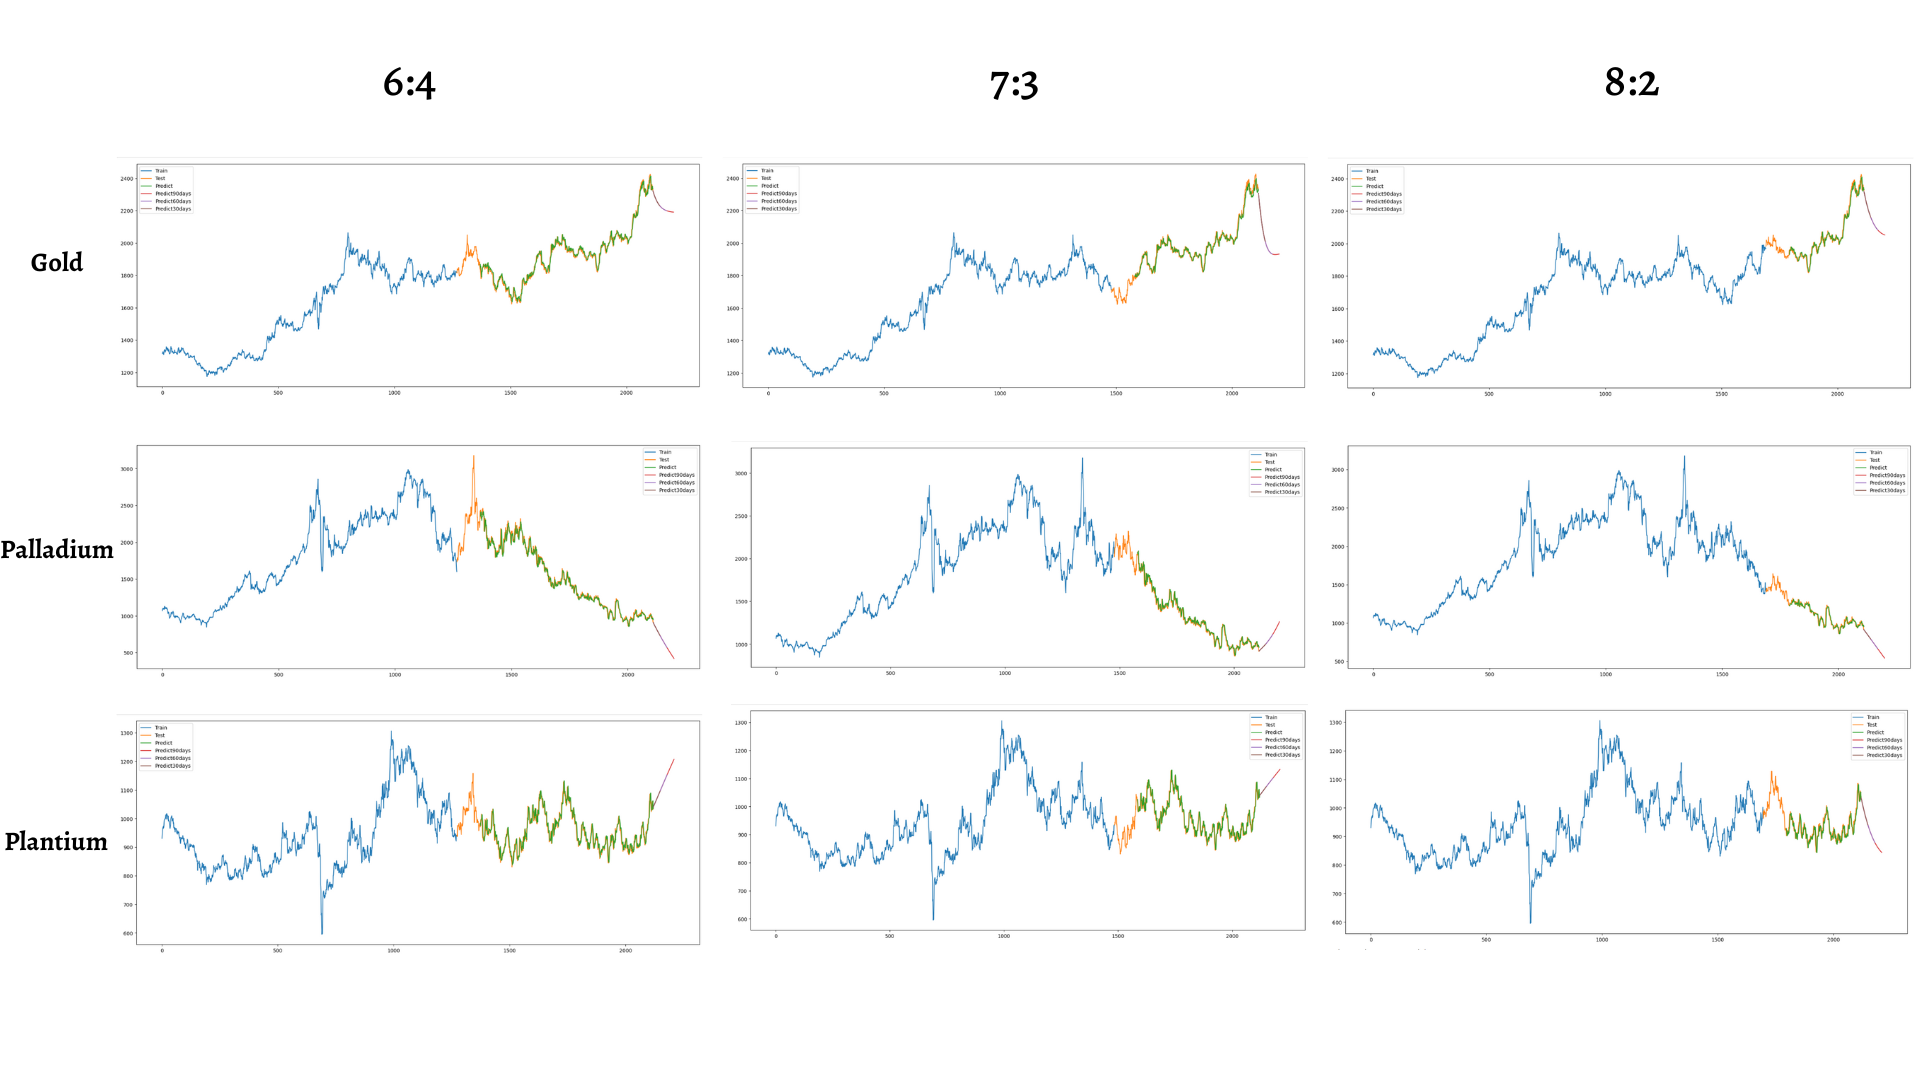
\includegraphics[width=0.5\textwidth]{img/GRU_result.png}}
\caption{Kết quả thực nghiệm GRU}
\label{fig}
\end{figure}

LSTM – là 1 dạng đặc biệt của mô hình RNN (Recurrent Neural Network), có khả năng học được các phụ thuộc. Phương pháp chính của mô hình LSTM là trạng thái tế bào (cell state), nó tương tự như 1 băng truyền chạy xuyên suốt tất cả các mắt xích và tương tác tuyến tính với các mắt xích đó vì vậy mà các thông tin dễ dàng truyền đi thông suốt mà không sợ bị thay đổi. LSTM sở hữu khả năng chọn lọc thông tin quan trọng bằng cách loại bỏ hoặc thêm vào trạng thái (state) của nó. Quá trình này được kiểm soát bởi các cấu trúc được gọi là cổng (gate). Mỗi cổng hoạt động như một bộ lọc thông tin, quyết định lượng thông tin được phép đi qua. Cụ thể, cổng bao gồm một lớp mạng sigmoid, tạo ra một giá trị trong khoảng từ 0 đến 1, đại diện cho tỷ lệ thông tin được truyền qua. Giá trị 0 nghĩa là không có thông tin nào được truyền qua, trong khi giá trị 1 cho phép tất cả thông tin đi qua. LSTM sử dụng ba cổng như vậy để quản lý và điều chỉnh trạng thái của tế bào: cổng quên (forget gate), cổng vào (input gate) và cổng ra (output gate).

\begin{figure}[htbp]
\centerline{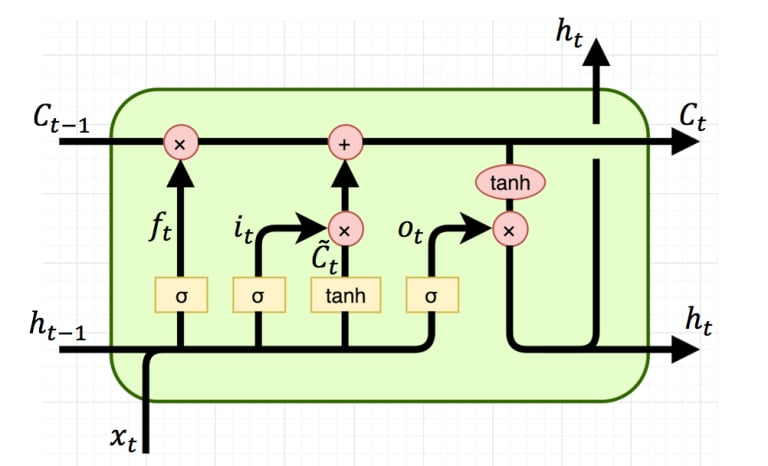
\includegraphics[width=0.4\textwidth]{img/LSTM.jpg}}
\caption{Kiến trúc LMST.}
\label{fig}
\end{figure}

Là phương pháp mô hình hóa biến thiên 2D theo thời gian để phân tích chuỗi thời gian tổng quát. Hành động tách các khoảng thời gian khác nhau khỏi chuỗi thời gian có thể làm giảm đáng kể độ phức tạp để xử lý các mô hình. Ngoài ra, FFT (Fast Fourier Transform) giúp nắm bắt được sự thay đổi trong và giữa các thời kỳ. Quá trình này cho phép chuỗi thời gian được tách rời có cách diễn giải vật lý rõ ràng hơn, nâng cao khả năng diễn giải của mô hình.

\begin{figure}[htbp]
\centerline{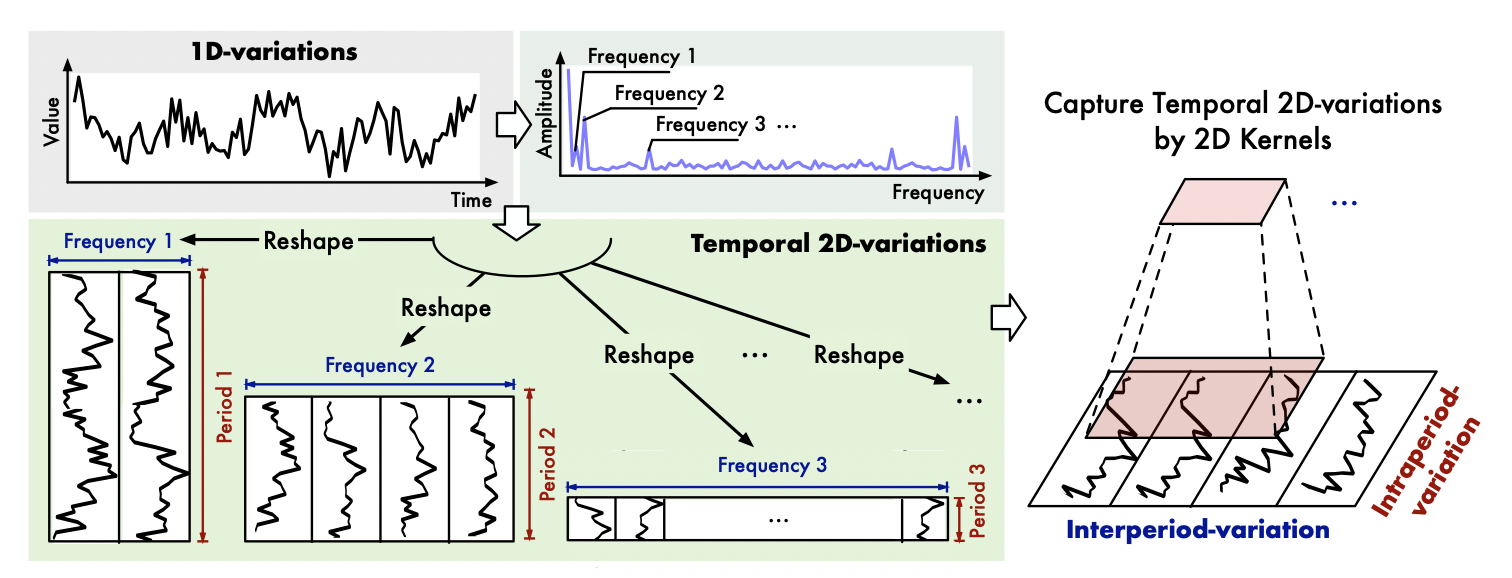
\includegraphics[width=0.4\textwidth]{img/2Dstructure.png}}
\caption{Minh họa cấu trúc 2D trong chuỗi thời gian.}
\label{fig}
\end{figure}

Bằng cách chuyển đổi dữ liệu chuỗi thời gian 1D thành một tập hợp các tensor 2D dựa trên nhiều chu kỳ, TimesNet phá vỡ giới hạn của chuỗi thời gian 1D và cho phép mô hình nắm bắt được sự biến đổi 2D theo thời gian của chuỗi thời gian.

\begin{figure}[htbp]
\centerline{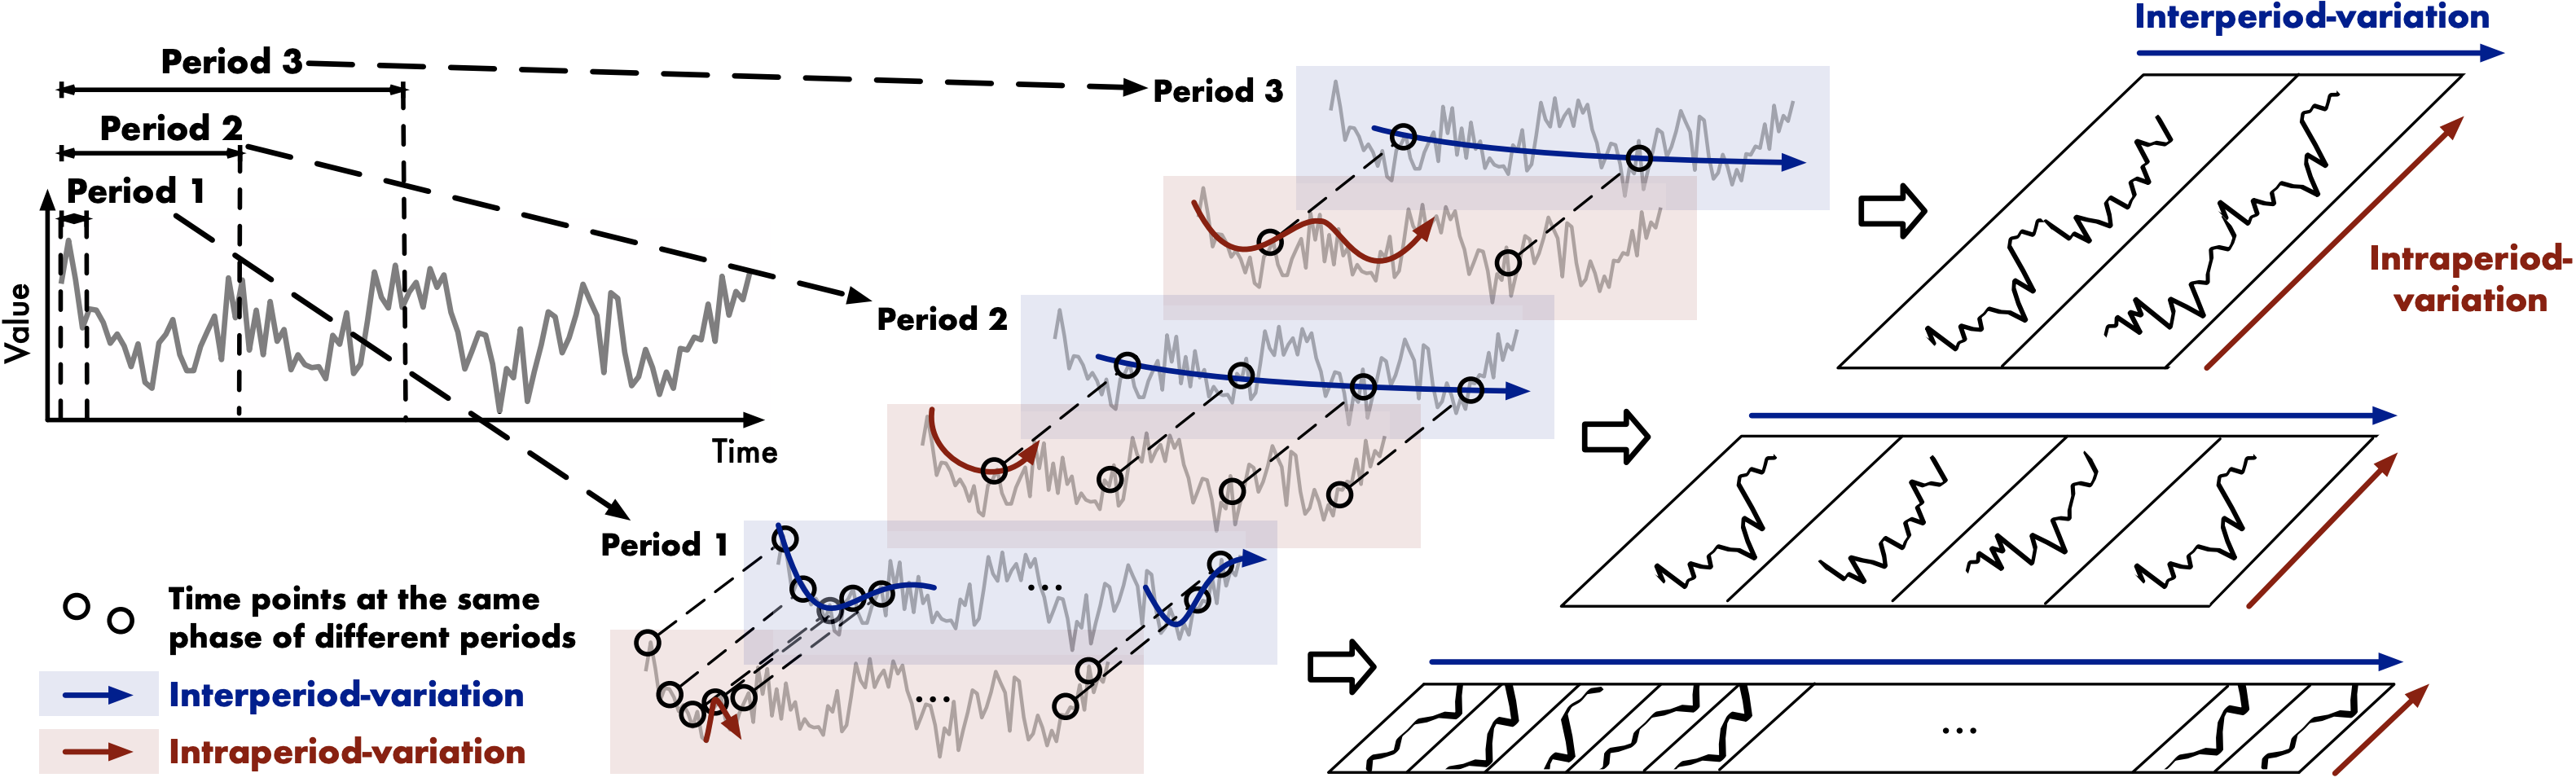
\includegraphics[width=0.4\textwidth]{img/2Dtensor.png}}
\caption{Chuyển đổi chuỗi thời gian 1D ban đầu thành một tập hợp các tensor 2D dựa trên nhiều chu kỳ.}
\label{fig}
\end{figure}

Autoformer: Phát triển từ Transformer, Autoformer như một kiến trúc phân rã mới với cơ chế Tự tương quan (Auto-corelation). Autoformer phá vỡ quy ước tiền xử lý về phân tách chuỗi và đổi mới nó thành khối bên trong cơ bản của các mô hình sâu. Thiết kế này trao quyền cho Autoformer khả năng phân rã lũy tiến cho chuỗi thời gian phức tạp. Hơn nữa, lấy cảm hứng từ lý thuyết quá trình ngẫu nhiên, mô hình này có cơ chế Tự tương quan dựa trên tính tuần hoàn của chuỗi, cơ chế này tiến hành khám phá phụ thuộc và tổng hợp biểu diễn ở cấp độ chuỗi phụ. Tự động tương quan vượt trội hơn khả năng tự chú ý cả về hiệu quả và độ chính xác. Trong dự báo dài hạn, Autoformer mang lại độ chính xác cao nhất, với mức cải thiện tương đối 38\% trên sáu điểm chuẩn, bao gồm năm ứng dụng thực tế: năng lượng, giao thông, kinh tế, thời tiết và bệnh tật.

\section{ĐỐI TƯỢNG NGHIÊN CỨU}
\subsection{BỘ DỮ LIỆU}
Bộ dữ liệu cung cấp thông tin chi tiết dữ liệu giá của 3 kim loại quý, cụ thể là Vàng, Bạch Kim và Palladi trong giai đoạn từ 01/03/2019 đến 26/03/2024. Dữ liệu bao gồm các cột: Ngày (Date), Giá mở cửa (Open), Giá đóng cửa (Close), Giá cao nhất (High), Giá thấp nhất (Low). Do mục tiêu là dự báo giá đóng cửa nên chỉ xử lý dữ liệu liên quan đến cột “Close”.

\subsection{MÔ TẢ THỐNG KÊ}
\begin{table}[htbp]
  \centering
\begin{tabular}{|c|c|c|c|}
    \hline
     \  & Gold & Palladium & Platinum \\ \hline
     Count & 1694 & 1687& 1695\\ \hline
     Mean & 1780,64 & 1888,11 & 958,24\\ \hline
     Std & 197,721 & 507,233 & 105,894\\ \hline
     Min & 1270,65 & 859,5 & 595\\ \hline
     25\% & 1708,035 & 1467 & 892\\ \hline
     50\% & 1811,18 & 1927,5 & 943,5\\ \hline
     75\% & 1923,6 & 2294,25 & 1018,5\\ \hline
     Max & 2202,2 & 3178 & 1306\\ \hline
\end{tabular}
\caption{Mô tả thống kê của vàng, paladi và bạch kim}
\end{table}

\begin{figure}[htbp]
\centerline{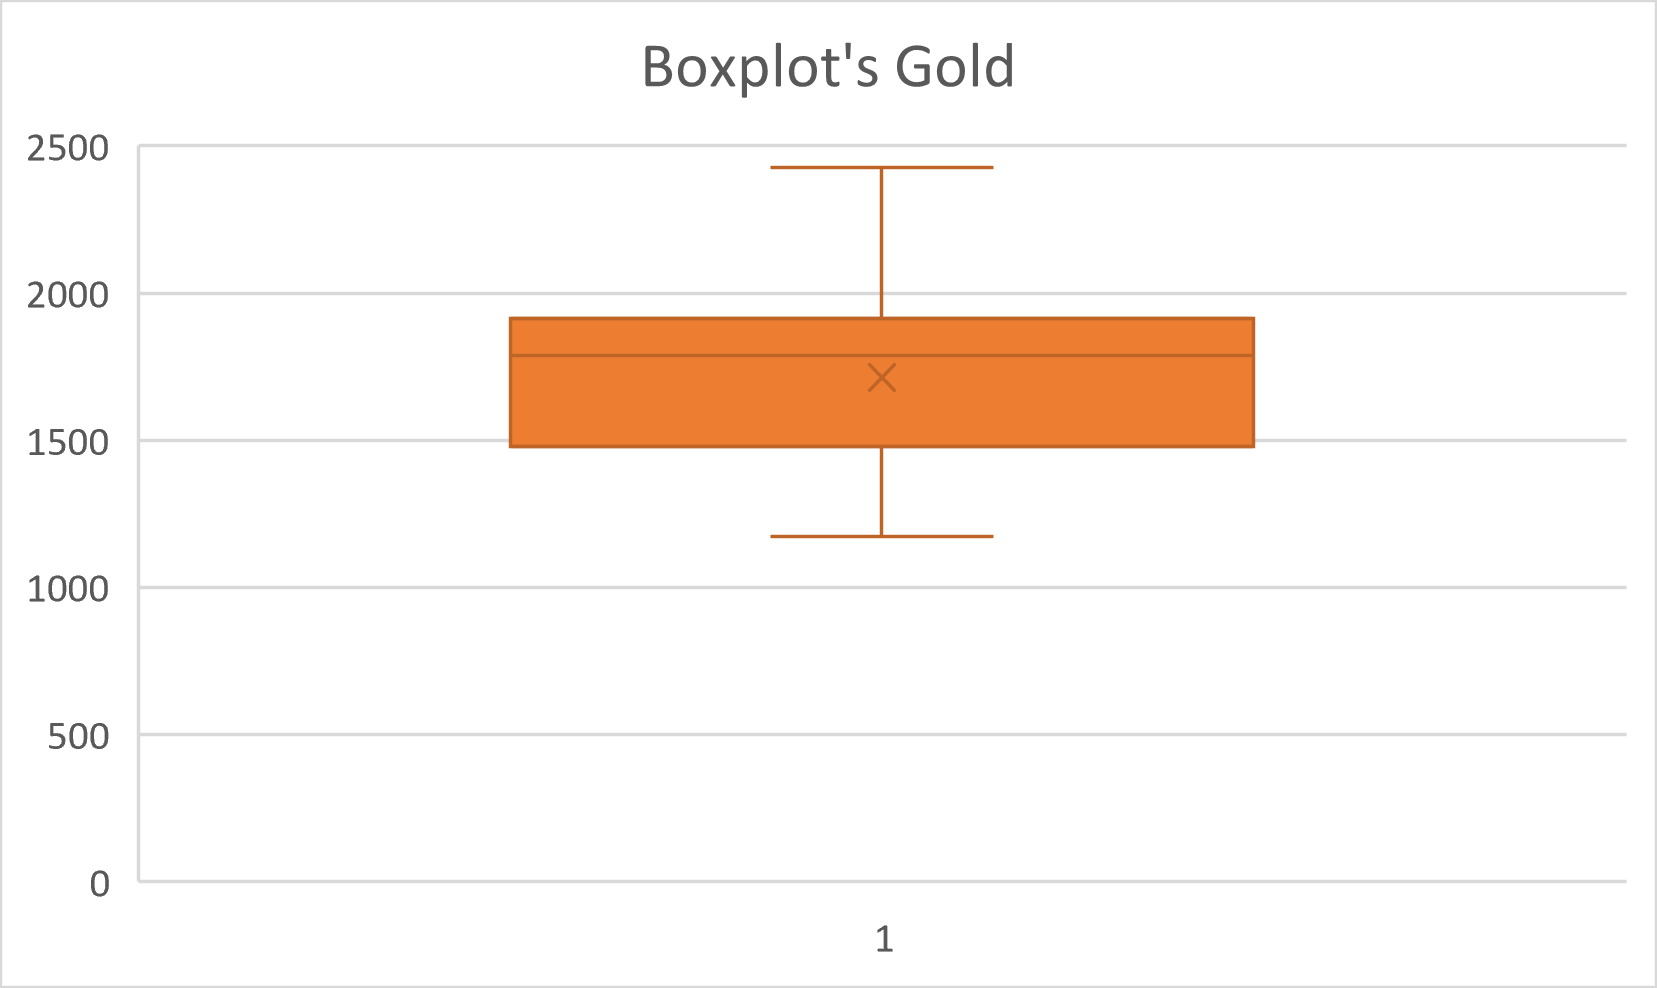
\includegraphics[width=0.4\textwidth]{img/Picture2.png}}
\caption{Sơ đồ boxplot của vàng}
\label{fig}
\end{figure}

\begin{figure}[htbp]
\centerline{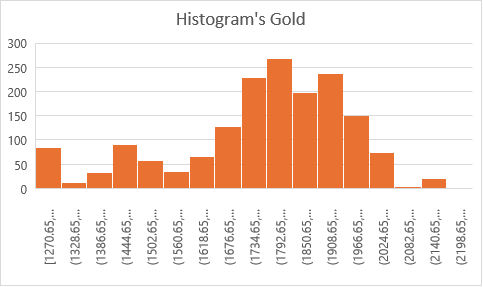
\includegraphics[width=0.4\textwidth]{img/Picture5.png}}
\caption{Sơ đồ histogram của vàng}
\label{fig}
\end{figure}

\begin{figure}[htbp]
\centerline{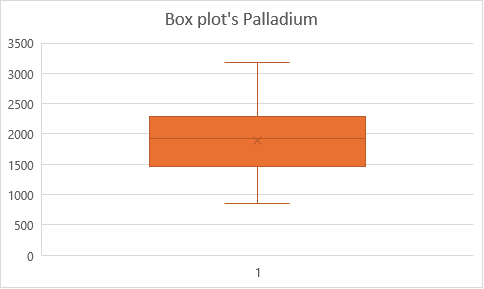
\includegraphics[width=0.4\textwidth]{img/Picture3.png}}
\caption{Sơ đồ boxplot của Paladi}
\label{fig}
\end{figure}

\begin{figure}[htbp]
\centerline{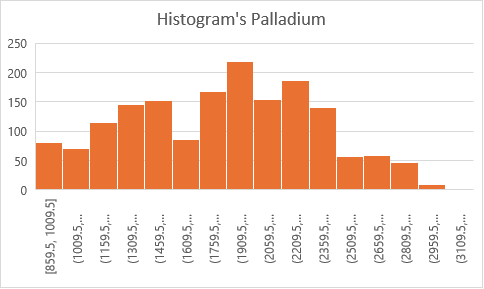
\includegraphics[width=0.4\textwidth]{img/Picture6.png}}
\caption{Sơ đồ histogram của Paladi}
\label{fig}
\end{figure}

\begin{figure}[htbp]
\centerline{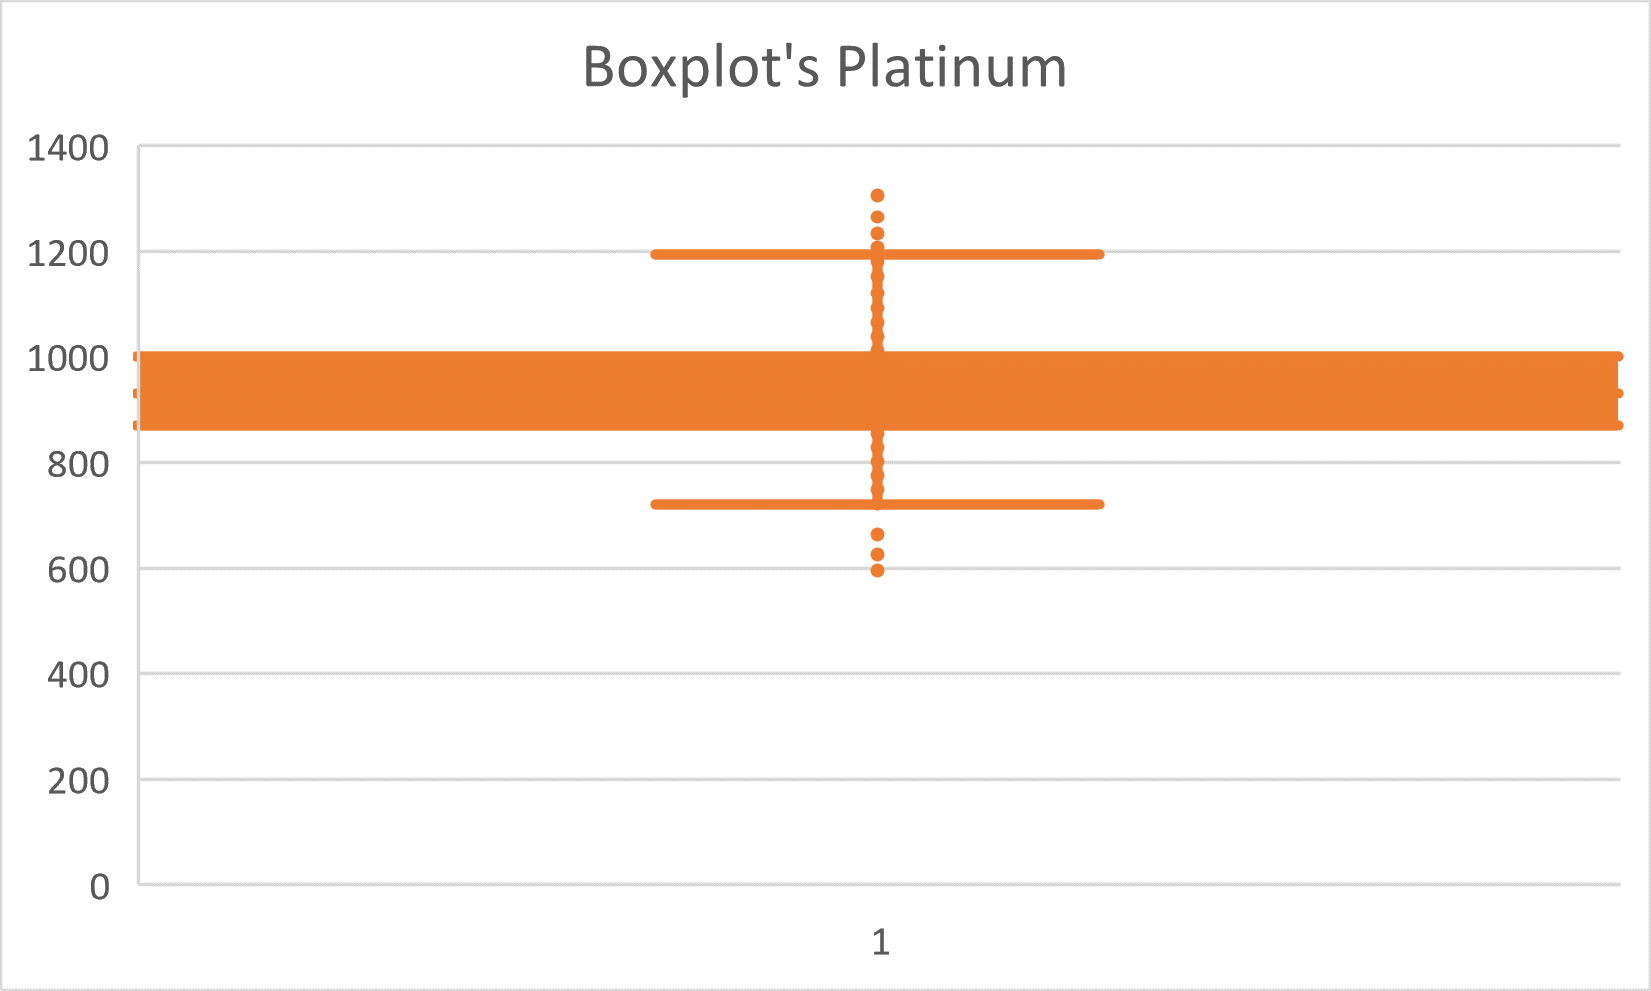
\includegraphics[width=0.4\textwidth]{img/Picture4.png}}
\caption{Sơ đồ boxplot của bạch kim}
\label{fig}
\end{figure}

\begin{figure}[htbp]
\centerline{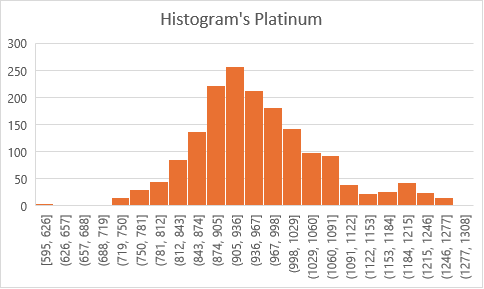
\includegraphics[width=0.4\textwidth]{img/Picture7.png}}
\caption{Sơ đồ histogram của bạch kim}
\label{fit}
\end{figure}

\section{PHƯƠNG PHÁP NGHIÊN CỨU}
\subsection{LINEAR REGRESSION (LR)}
Dự báo giá vàng bằng ARIMA, RW, ARFIMA, ETS, TBATS và MLR. Nghiên cứu của Alessio Azzutti\cite{azzu} , so sánh kết quả thu được từ 6 mô hình dự báo, để dự báo giá vàng. Nghiên cứu gồm 36 phạm vi dự báo khác nhau cả về dài hạn và ngắn hạn, từ kết quả thu được ta nhận thấy không có mô hình nào trong 6 mô hình có thể đưa ra dự báo chính xác nhất về giá vàng trong cả ngắn hạn và dài hạn. Tuy nhiên dựa trên RMSE thì ARIMA cung cấp dự báo tốt hơn lần lượt là 5\%, 2\%, 1\%, 54\% và 55\% so với mô hình RW, ETS, TBATS, ARFIMA và MLR.

\subsection{ETS}
\begin{figure}[htbp]
\centerline{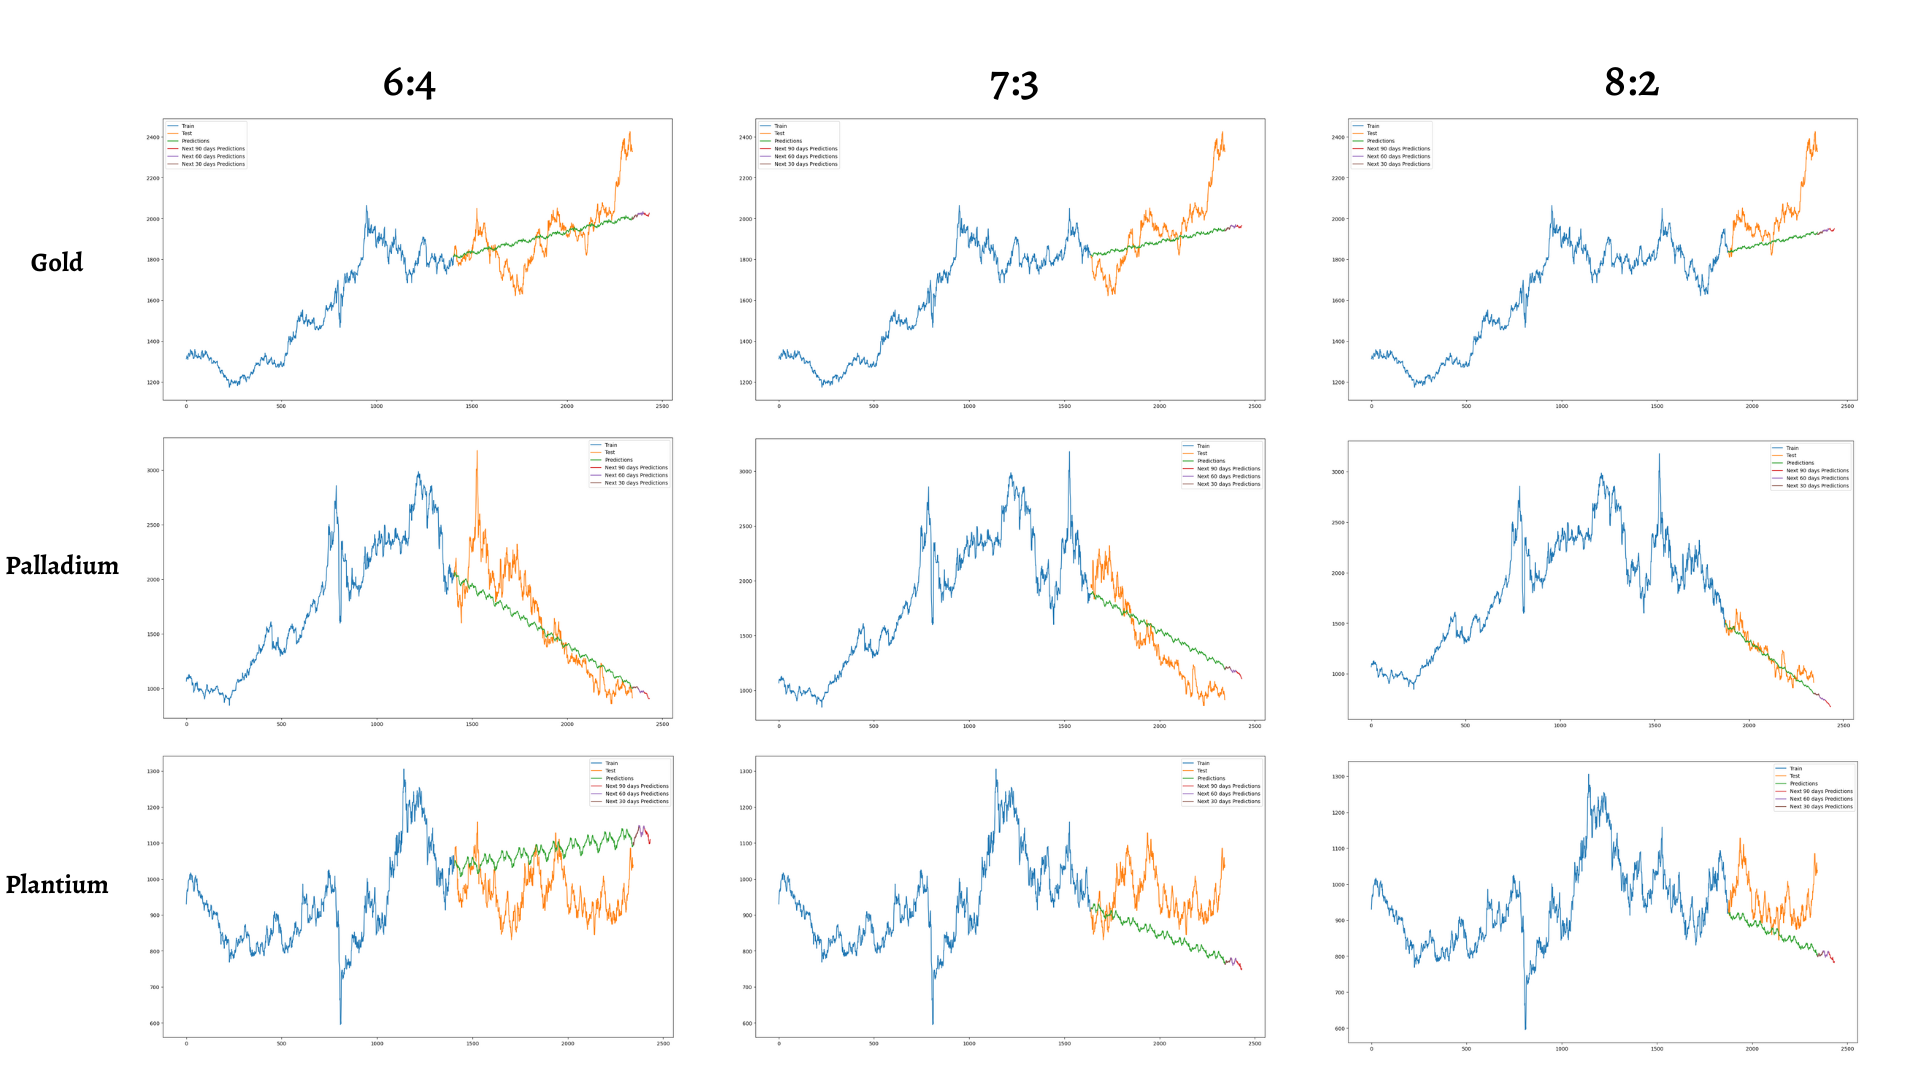
\includegraphics[width=0.5\textwidth]{img/ETS_result.png}}
\caption{Kết quả thực nghiệm ETS}
\label{fig}
\end{figure}

\subsection{ARIMA}
Dự đoán giá vàng sử dụng mô hình ARIMA được nghiên cứu bởi Banhi Guha và Gautam Bandyopadhyay\cite{article2}. Trong nghiên cứu này, họ đã phân tích hiệu suất giá vàng trong 10 năm qua. Dựa trên giá được giao dịch trên MCX, trong sáu bộ tham số mô hình khác nhau cho thấy ARIMA(1,1,1) là mô hình dự đoán tốt nhất cho các giá trị tương lai của vàng và đáp ứng được tất cả các tiêu chí thống kê phù hợp.

\subsection{Random Forest (RF)}
\begin{figure}[H]
\centerline{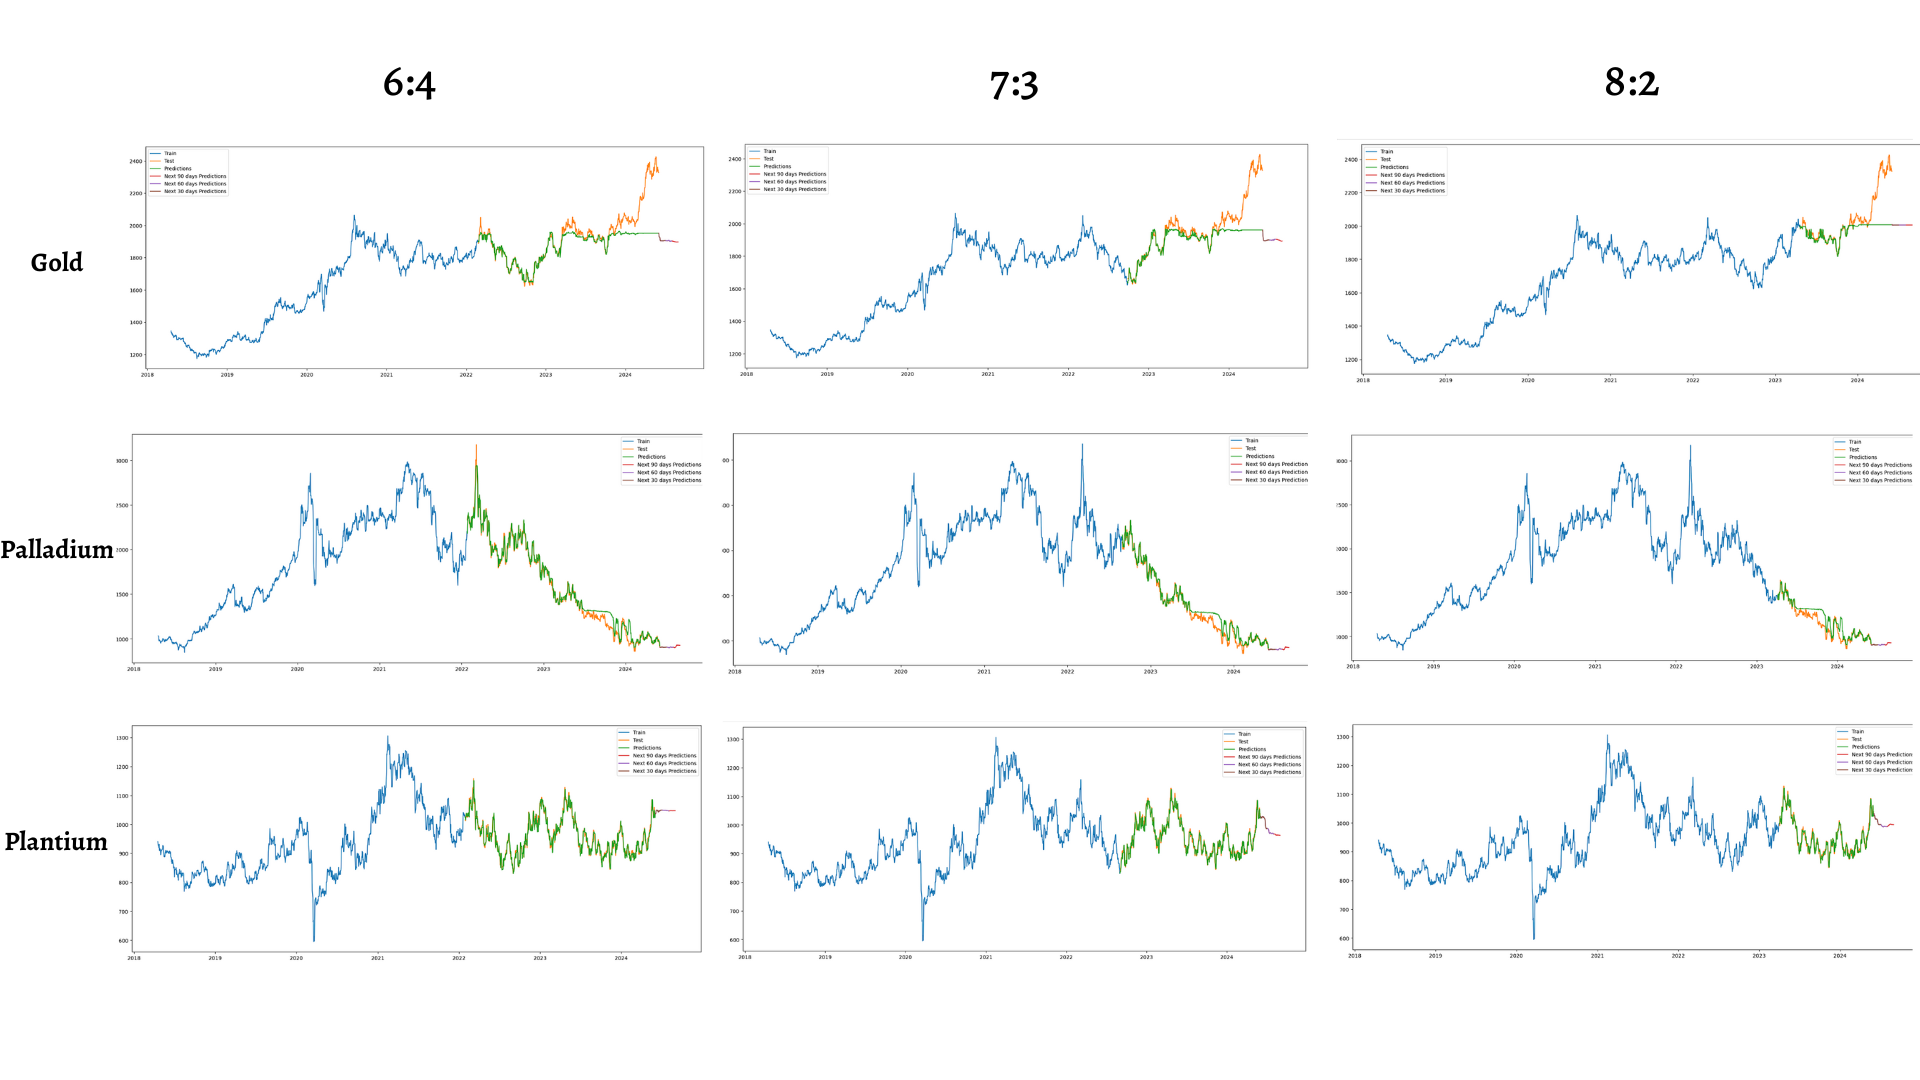
\includegraphics[width=0.45\textwidth]{img/RF_result.png}}
\caption{Kết quả thực nghiệm Random Forest}
\label{fig}
\end{figure}

\subsection{Support Vector Regression (SVR)}
SVR (Support Vector Regression) là một một biến thể của phương pháp máy vector hỗ trợ (Support Vector Machines - SVM) được sử dụng cho các bài toán hồi quy. SVR sẽ tìm một hàm hồi quy tốt nhất mà sai số của các dự đoán nằm trong khoảng chấp nhận được. SVR có thể sử dụng các hàm hạt nhân(kernel) để chuyển đổi không gian đầu vào sang không gian đặc trưng cao giúp cho việc xử lý các dữ liệu tuyến tính và phi tuyến. Một kernel tuyến tính là tích vô hướng đơn giản giữa hai vector đầu vào, trong khi một kernel phi tuyến là một hàm phức tạp hơn có thể nắm bắt các mẫu phức tạp hơn trong dữ liệu. 

Không giống như các mô hình hồi quy truyền thống, SVR tập trung vào việc giảm thiểu lỗi dự đoán thay vì khớp dữ liệu một cách chính xác. Để đạt được điều này bằng cách tìm một siêu phẳng tối ưu tối ưu hóa khoảng cách hay biên, giữa các giá trị dự đoán và các điểm dữ liệu thực tế. SVR đạt được sự cân bằng giữa tính đơn giản và tính linh hoạt bằng cách cho phép một mức đúng sai nhất định, hay biên độ lỗi, xung quanh các giá trị dự đoán.


Hàm hồi quy trong SVR:
\[
f(x) = \langle w, x \rangle + b
\]\\
Hàm mất mát E-insensitive:
\[
L(y, F(x_i, \hat{w})) = \max(0, y - F(x_i, \hat{w}) - \varepsilon)
\]\\
Trong đó:\\
    \indent\textbullet\ \(L(y,F(x_i,\hat{w})\): hàm lỗi.\\
    \indent\textbullet\ \(y\): giá trị thực.\\
    \indent\textbullet\ \(F(x_i,\hat{w})\): sai số ngẫu nhiên.\\
    \indent\textbullet\ \(\varepsilon\): tham số điều chỉnh cho phép sai lệch.\\
Dưới đây là một số hàm kernel có thể sử dụng trong SVM
\begin{table}[htbp]
  \centering
\begin{tabular}{|c|c|}
    \hline
     Kernel& Hàm\\ \hline
     Linear &  $f(X1,X2)=X1^TX2$\\ \hline
     Polynomial & $f(X1,X2)=(X1^TX2 +1)^d$ \\ \hline
     Sigmoid &  $f(X1,X2)=\tanh(\alpha x^{T}y+x)$\\ \hline
     RBF &  $f(X1,X2)=e^{\frac{-{\mid\mid x1-x2 \mid\mid}^2}{2\sigma^2}}$\\ \hline
\end{tabular}
\end{table}\\
\textbf{Linear}: Đây là kernel đơn giản nhất và cơ bản nhất trong SVR. Linear phù hợp khi dữ liệu có thể được phân tách tuyến tính trong không gian đầu vào.\\
\textbf{Polynomial}: Kernel này biến đổi dữ liệu đầu vào không gian đa thức, được xác định bởi tham số bậc và hệ số độ lệch.\\
\textbf{Sigmoid}: Kernel này biến đổi dữ liệu đầu vào thành không gian phi tuyến bằng cách sử dụng hàm sigmoid. Hàm sigmoid áp dụng phép biến đổi phi tuyến lên tích vô hướng của hai vector đầu vào. Ngoài ra có thể được sử dụng cho các bài toán có dữ liệu nhị phân.\\
\textbf{RBF}: Đây là kernel phi tuyến phổ biến và cho phép mô hình học các cấu trúc phi tuyến phức tạp. Hàm RBF được xác định bởi tham số độ dốc\\

\subsection{Recurrent Neural Network (RNN)}
Madini O. Alassafi, Mutasem Jarrah, Reem Alotaibi\cite{10263962} đã sử dụng mô hình RNN và LSTM  để dự đoán sự lây lan của COVID-19 ở Malaysia, Morocco và Ả Rập Xê Út. Nghiên cứu cũng so sánh số ca mắc bệnh và số ca tử vong do COVID-19 ở Malaysia, Morocco và Ả Rập Xê Út. Sau đó, họ dự đoán số ca mắc và tử vong trong 7 ngày tiếp theo dựa trên dữ liệu có sẵn đến ngày 3 tháng 12 năm 2020. Kết quả độ chính xác của các mô hình lần lượt là 97.34\% RNN (Sigmoid), 93.32\% RNN (Tanh) và 99.27\% LSTM (ReLU). 

\subsection{Gated Recurrent Unit (GRU)}
\begin{figure}[htbp]
\centerline{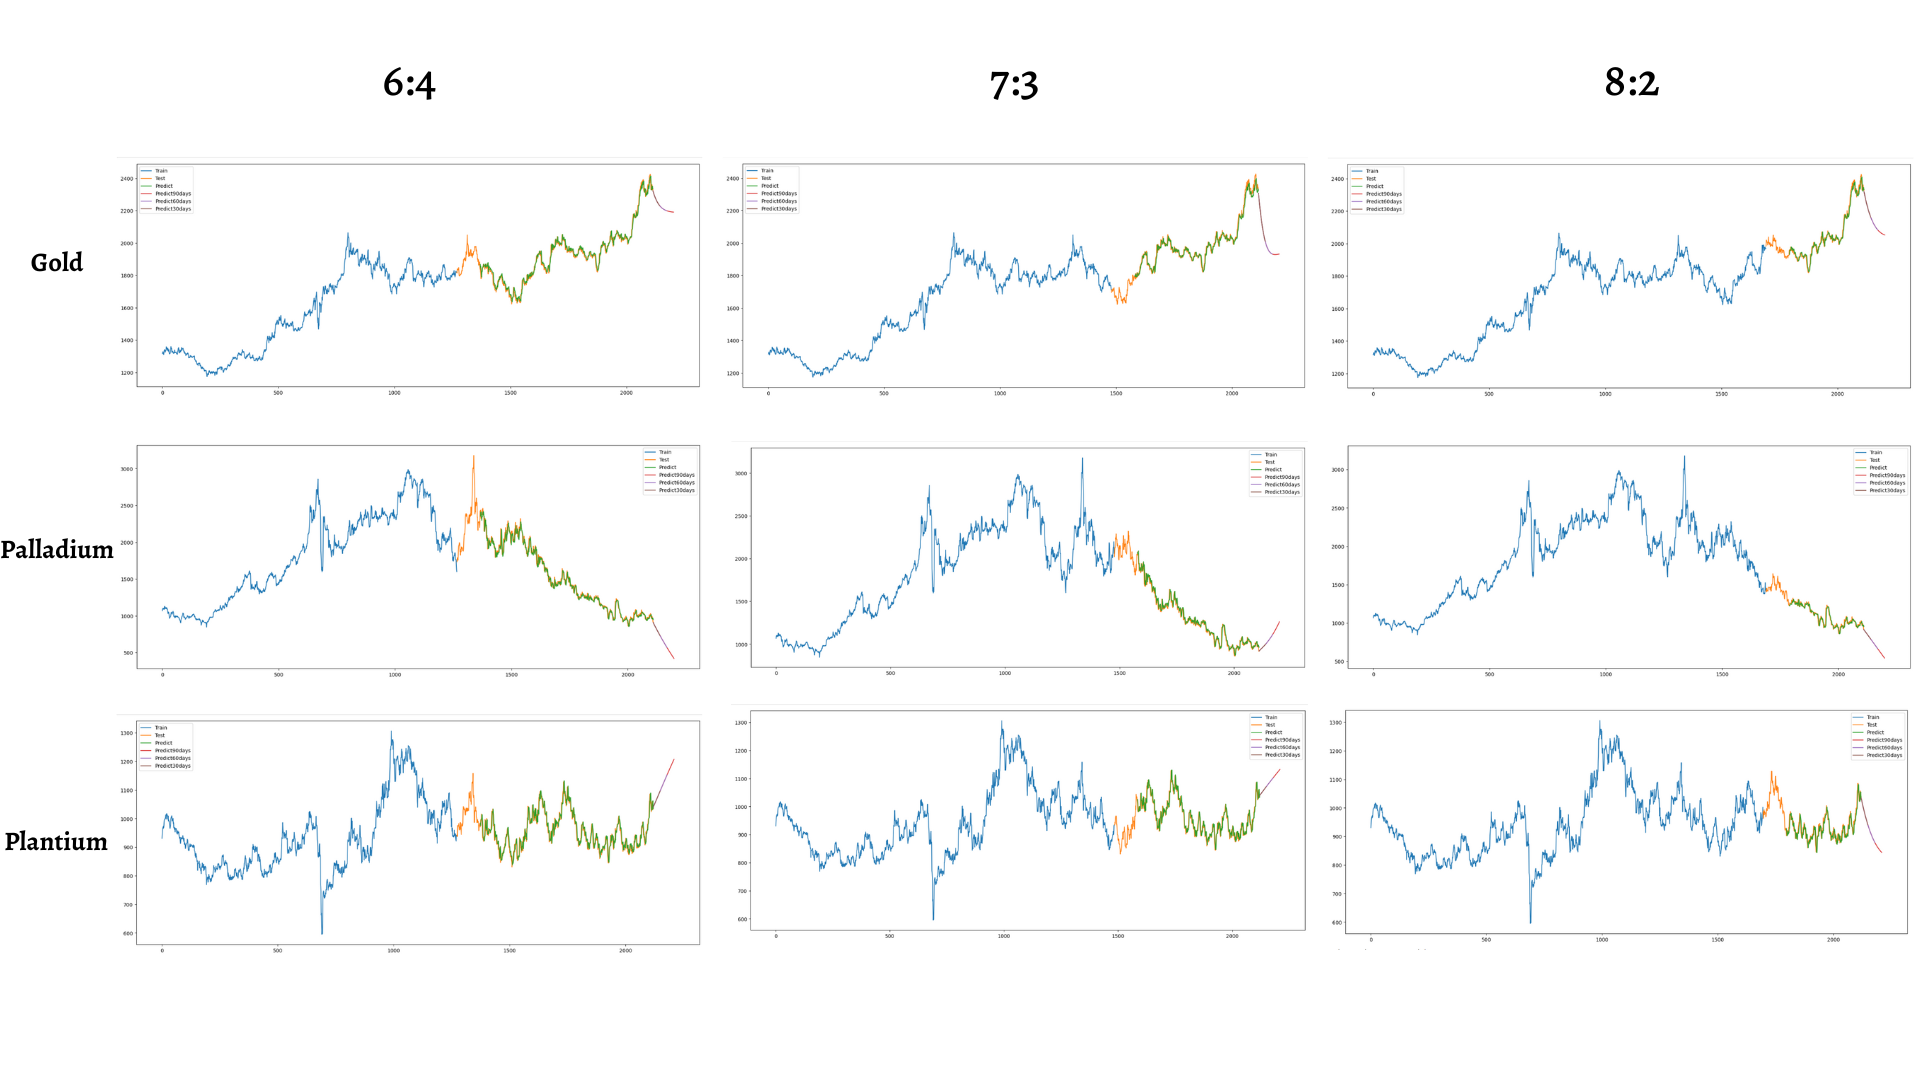
\includegraphics[width=0.5\textwidth]{img/GRU_result.png}}
\caption{Kết quả thực nghiệm GRU}
\label{fig}
\end{figure}

\subsection{Long Short Term Memory (LSTM)}
LSTM – là 1 dạng đặc biệt của mô hình RNN (Recurrent Neural Network), có khả năng học được các phụ thuộc. Phương pháp chính của mô hình LSTM là trạng thái tế bào (cell state), nó tương tự như 1 băng truyền chạy xuyên suốt tất cả các mắt xích và tương tác tuyến tính với các mắt xích đó vì vậy mà các thông tin dễ dàng truyền đi thông suốt mà không sợ bị thay đổi. LSTM sở hữu khả năng chọn lọc thông tin quan trọng bằng cách loại bỏ hoặc thêm vào trạng thái (state) của nó. Quá trình này được kiểm soát bởi các cấu trúc được gọi là cổng (gate). Mỗi cổng hoạt động như một bộ lọc thông tin, quyết định lượng thông tin được phép đi qua. Cụ thể, cổng bao gồm một lớp mạng sigmoid, tạo ra một giá trị trong khoảng từ 0 đến 1, đại diện cho tỷ lệ thông tin được truyền qua. Giá trị 0 nghĩa là không có thông tin nào được truyền qua, trong khi giá trị 1 cho phép tất cả thông tin đi qua. LSTM sử dụng ba cổng như vậy để quản lý và điều chỉnh trạng thái của tế bào: cổng quên (forget gate), cổng vào (input gate) và cổng ra (output gate).

\begin{figure}[htbp]
\centerline{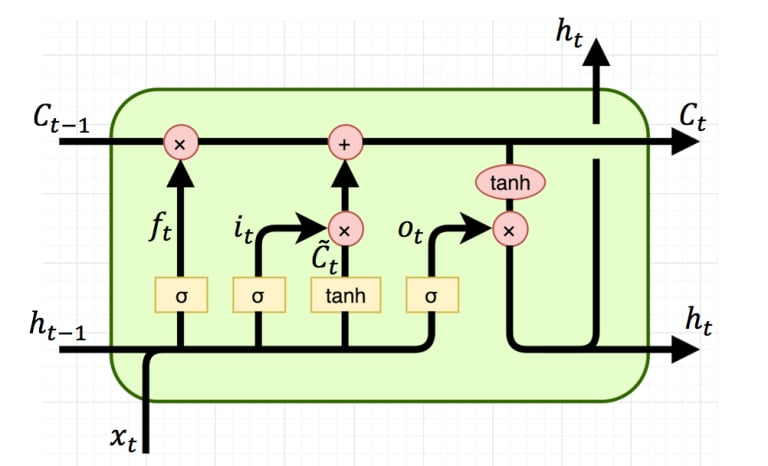
\includegraphics[width=0.4\textwidth]{img/LSTM.jpg}}
\caption{Kiến trúc LMST.}
\label{fig}
\end{figure}

\subsection{TimesNet}
Là phương pháp mô hình hóa biến thiên 2D theo thời gian để phân tích chuỗi thời gian tổng quát. Hành động tách các khoảng thời gian khác nhau khỏi chuỗi thời gian có thể làm giảm đáng kể độ phức tạp để xử lý các mô hình. Ngoài ra, FFT (Fast Fourier Transform) giúp nắm bắt được sự thay đổi trong và giữa các thời kỳ. Quá trình này cho phép chuỗi thời gian được tách rời có cách diễn giải vật lý rõ ràng hơn, nâng cao khả năng diễn giải của mô hình.

\begin{figure}[htbp]
\centerline{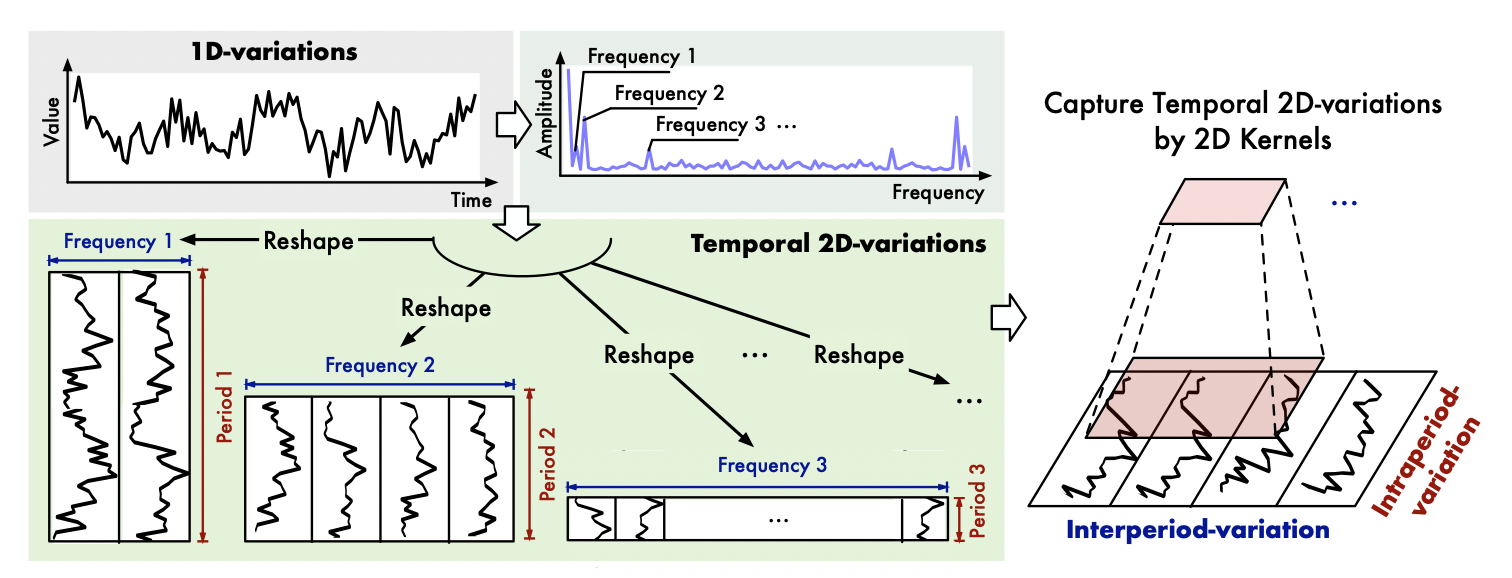
\includegraphics[width=0.4\textwidth]{img/2Dstructure.png}}
\caption{Minh họa cấu trúc 2D trong chuỗi thời gian.}
\label{fig}
\end{figure}

Bằng cách chuyển đổi dữ liệu chuỗi thời gian 1D thành một tập hợp các tensor 2D dựa trên nhiều chu kỳ, TimesNet phá vỡ giới hạn của chuỗi thời gian 1D và cho phép mô hình nắm bắt được sự biến đổi 2D theo thời gian của chuỗi thời gian.

\begin{figure}[htbp]
\centerline{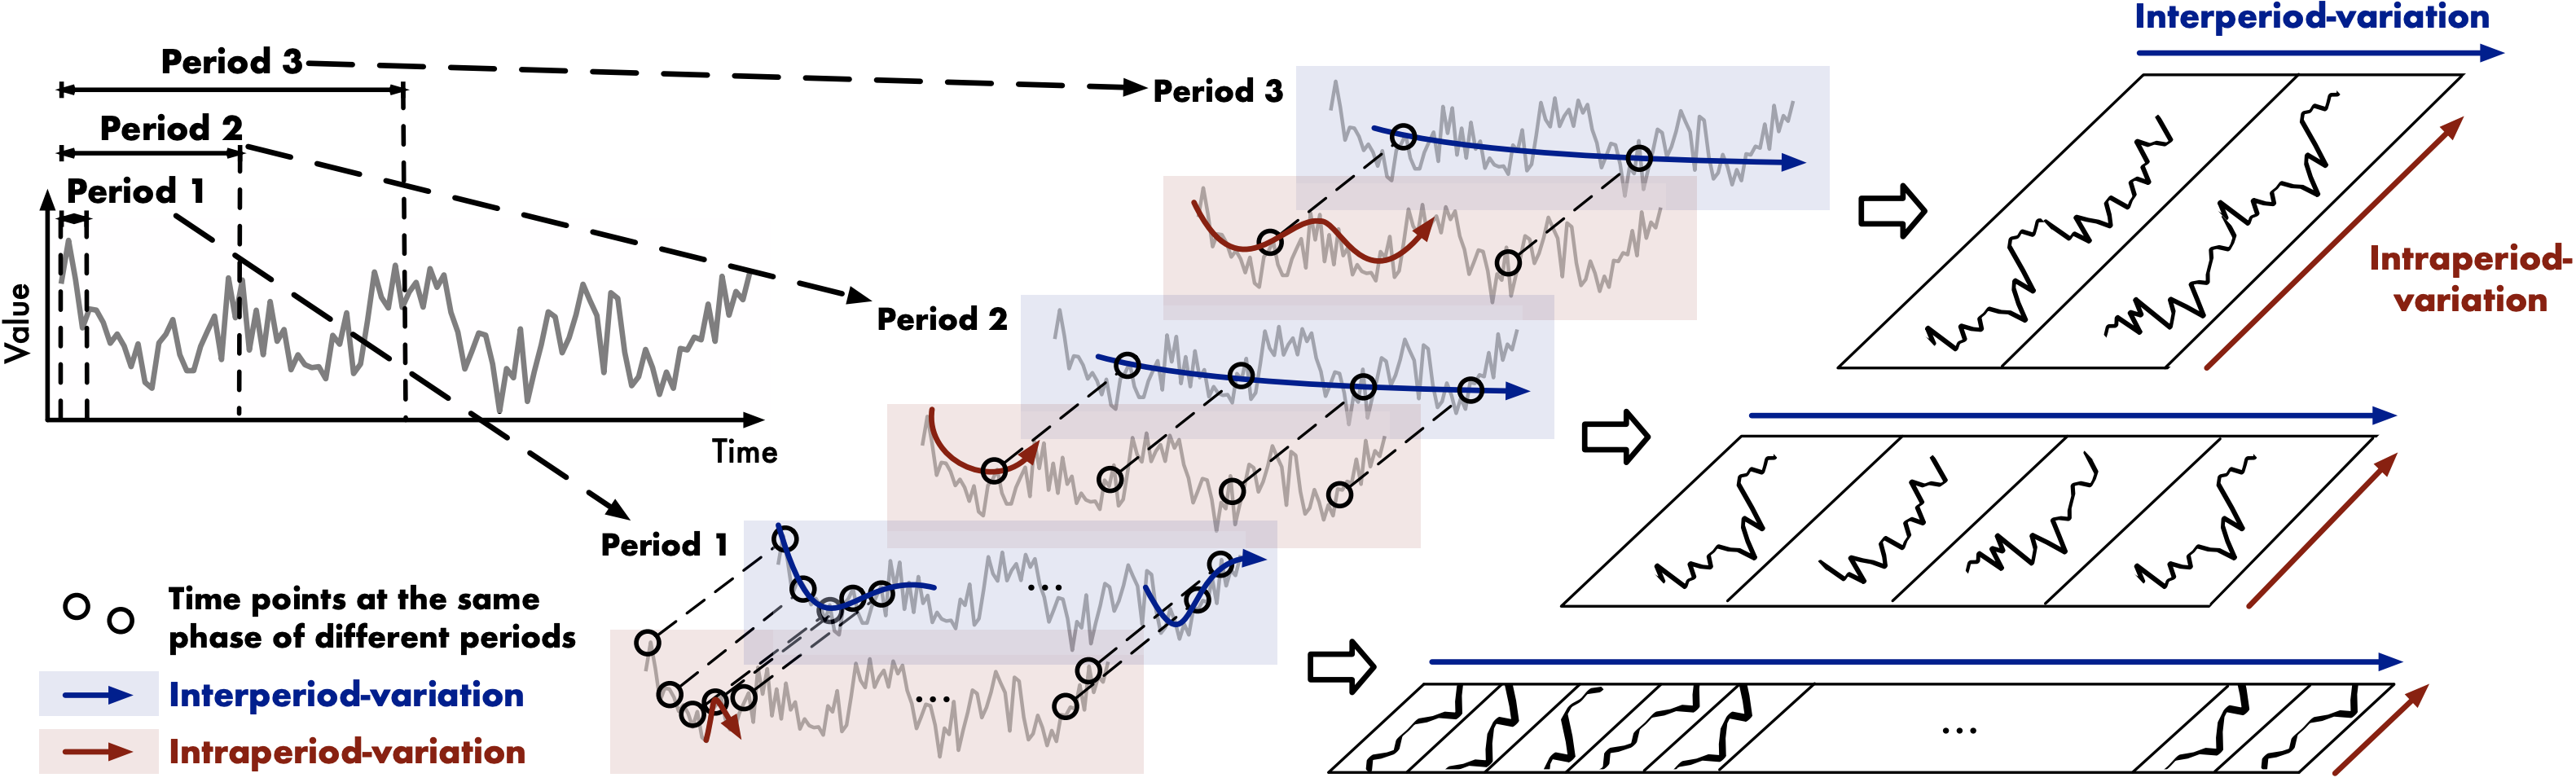
\includegraphics[width=0.4\textwidth]{img/2Dtensor.png}}
\caption{Chuyển đổi chuỗi thời gian 1D ban đầu thành một tập hợp các tensor 2D dựa trên nhiều chu kỳ.}
\label{fig}
\end{figure}

\subsection{Autoformer}
Autoformer: Phát triển từ Transformer, Autoformer như một kiến trúc phân rã mới với cơ chế Tự tương quan (Auto-corelation). Autoformer phá vỡ quy ước tiền xử lý về phân tách chuỗi và đổi mới nó thành khối bên trong cơ bản của các mô hình sâu. Thiết kế này trao quyền cho Autoformer khả năng phân rã lũy tiến cho chuỗi thời gian phức tạp. Hơn nữa, lấy cảm hứng từ lý thuyết quá trình ngẫu nhiên, mô hình này có cơ chế Tự tương quan dựa trên tính tuần hoàn của chuỗi, cơ chế này tiến hành khám phá phụ thuộc và tổng hợp biểu diễn ở cấp độ chuỗi phụ. Tự động tương quan vượt trội hơn khả năng tự chú ý cả về hiệu quả và độ chính xác. Trong dự báo dài hạn, Autoformer mang lại độ chính xác cao nhất, với mức cải thiện tương đối 38\% trên sáu điểm chuẩn, bao gồm năm ứng dụng thực tế: năng lượng, giao thông, kinh tế, thời tiết và bệnh tật.

\subsection{Độ đo}
Để đánh giá năng lực dự đoán của các mô hình sử dụng trong đồ án, nhóm sử dụng ba phép đo hiệu suất bao gồm: Mean Absolute Percentage Error (MAPE), Root Mean Square Error (RMSE) và Mean Square Error (MSE).

Độ đo MAPE đo lường sai số tuyệt đối trung bình giữa giá trị dự đoán và giá trị thực tế với công thức như sau:
\[
MAPE = \frac{\sum_{i=1}^{n}\left(\frac{abs(y_i - f_i)}{y_i}\right)}{n}
\]

Độ đo MSE tính toán trung bình bình phương của các sai số giữa giá trị thực tế và giá trị dự báo với công thức sau:
\[
MSE = \frac{\sum(f_i - y_i)^2}{N}
\]

Độ đo RMSE đo lường khoảng cách trung bình giữa các giá trị dự đoán và thực tế với công thức như sau:
\[
RMSE = \sqrt{\frac{\sum_{i=1}^{n}(f_i - y_i)^2}{n}}
\]
Trong đó:\\
    \indent\textbullet\ \(f_{i}\) là giá trị dự đoán cho mẫu thứ i.\\
    \indent\textbullet\ \(y_{i}\) là giá trị thực tế cho mẫu thứ i.\\
    \indent\textbullet\ \(N\) là số lượng mẫu.


\section{Thực nghiệm}
Dự báo giá vàng bằng ARIMA, RW, ARFIMA, ETS, TBATS và MLR. Nghiên cứu của Alessio Azzutti\cite{azzu} , so sánh kết quả thu được từ 6 mô hình dự báo, để dự báo giá vàng. Nghiên cứu gồm 36 phạm vi dự báo khác nhau cả về dài hạn và ngắn hạn, từ kết quả thu được ta nhận thấy không có mô hình nào trong 6 mô hình có thể đưa ra dự báo chính xác nhất về giá vàng trong cả ngắn hạn và dài hạn. Tuy nhiên dựa trên RMSE thì ARIMA cung cấp dự báo tốt hơn lần lượt là 5\%, 2\%, 1\%, 54\% và 55\% so với mô hình RW, ETS, TBATS, ARFIMA và MLR.

\begin{figure}[htbp]
\centerline{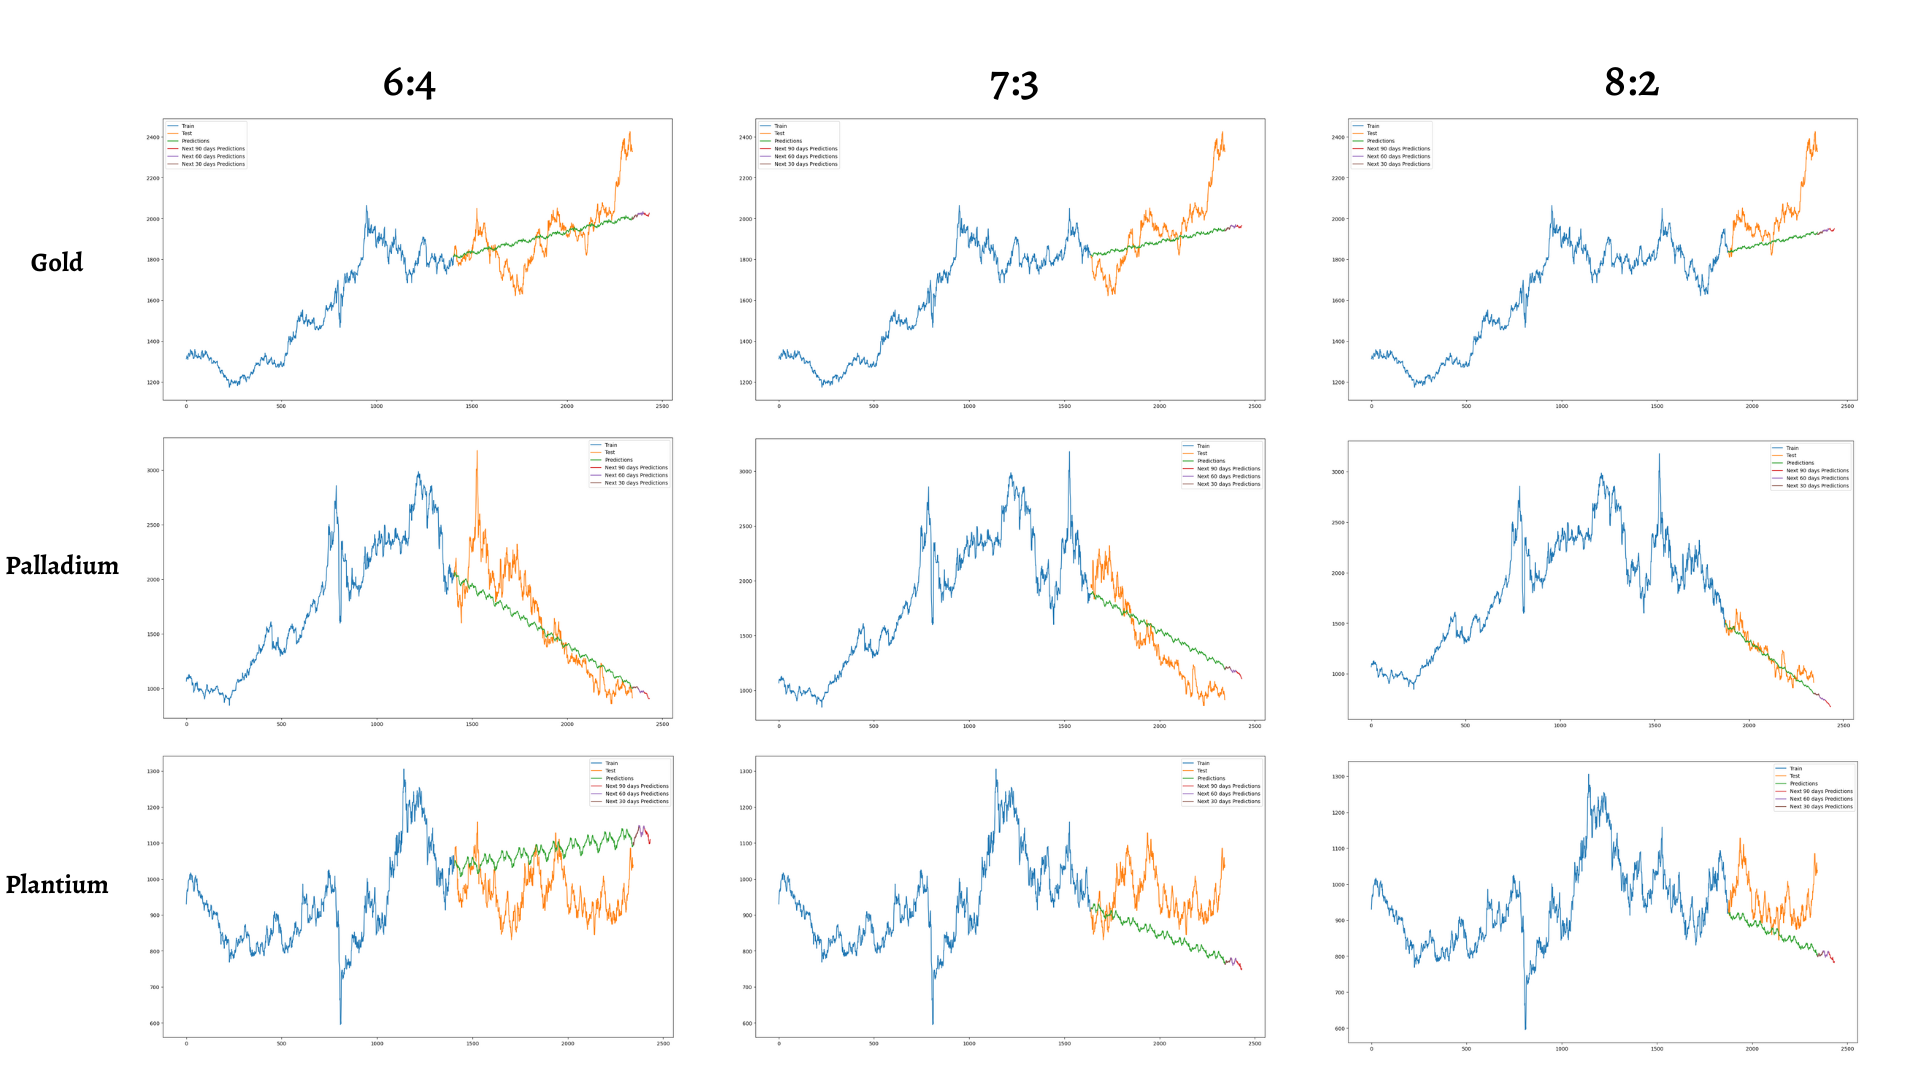
\includegraphics[width=0.5\textwidth]{img/ETS_result.png}}
\caption{Kết quả thực nghiệm ETS}
\label{fig}
\end{figure}

Dự đoán giá vàng sử dụng mô hình ARIMA được nghiên cứu bởi Banhi Guha và Gautam Bandyopadhyay\cite{article2}. Trong nghiên cứu này, họ đã phân tích hiệu suất giá vàng trong 10 năm qua. Dựa trên giá được giao dịch trên MCX, trong sáu bộ tham số mô hình khác nhau cho thấy ARIMA(1,1,1) là mô hình dự đoán tốt nhất cho các giá trị tương lai của vàng và đáp ứng được tất cả các tiêu chí thống kê phù hợp.

\begin{figure}[H]
\centerline{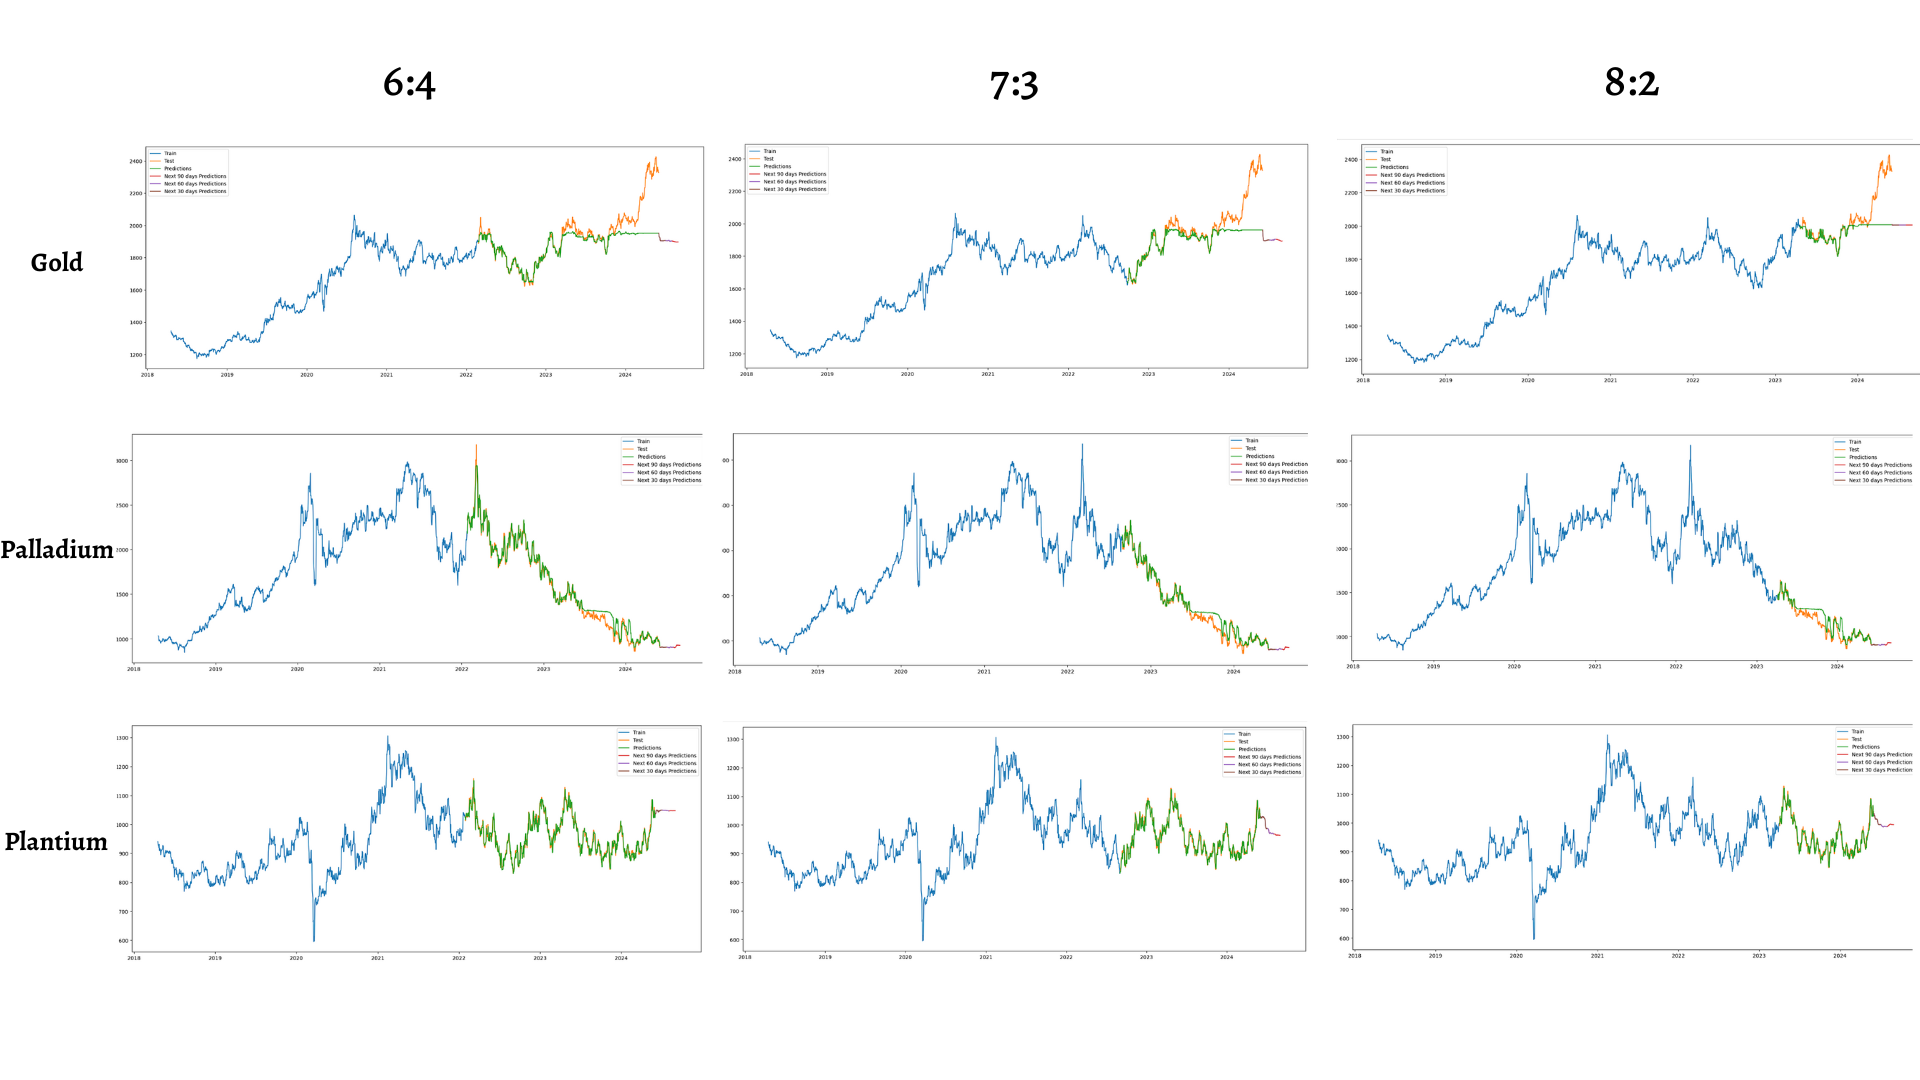
\includegraphics[width=0.45\textwidth]{img/RF_result.png}}
\caption{Kết quả thực nghiệm Random Forest}
\label{fig}
\end{figure}

\begin{figure}[H]
\centerline{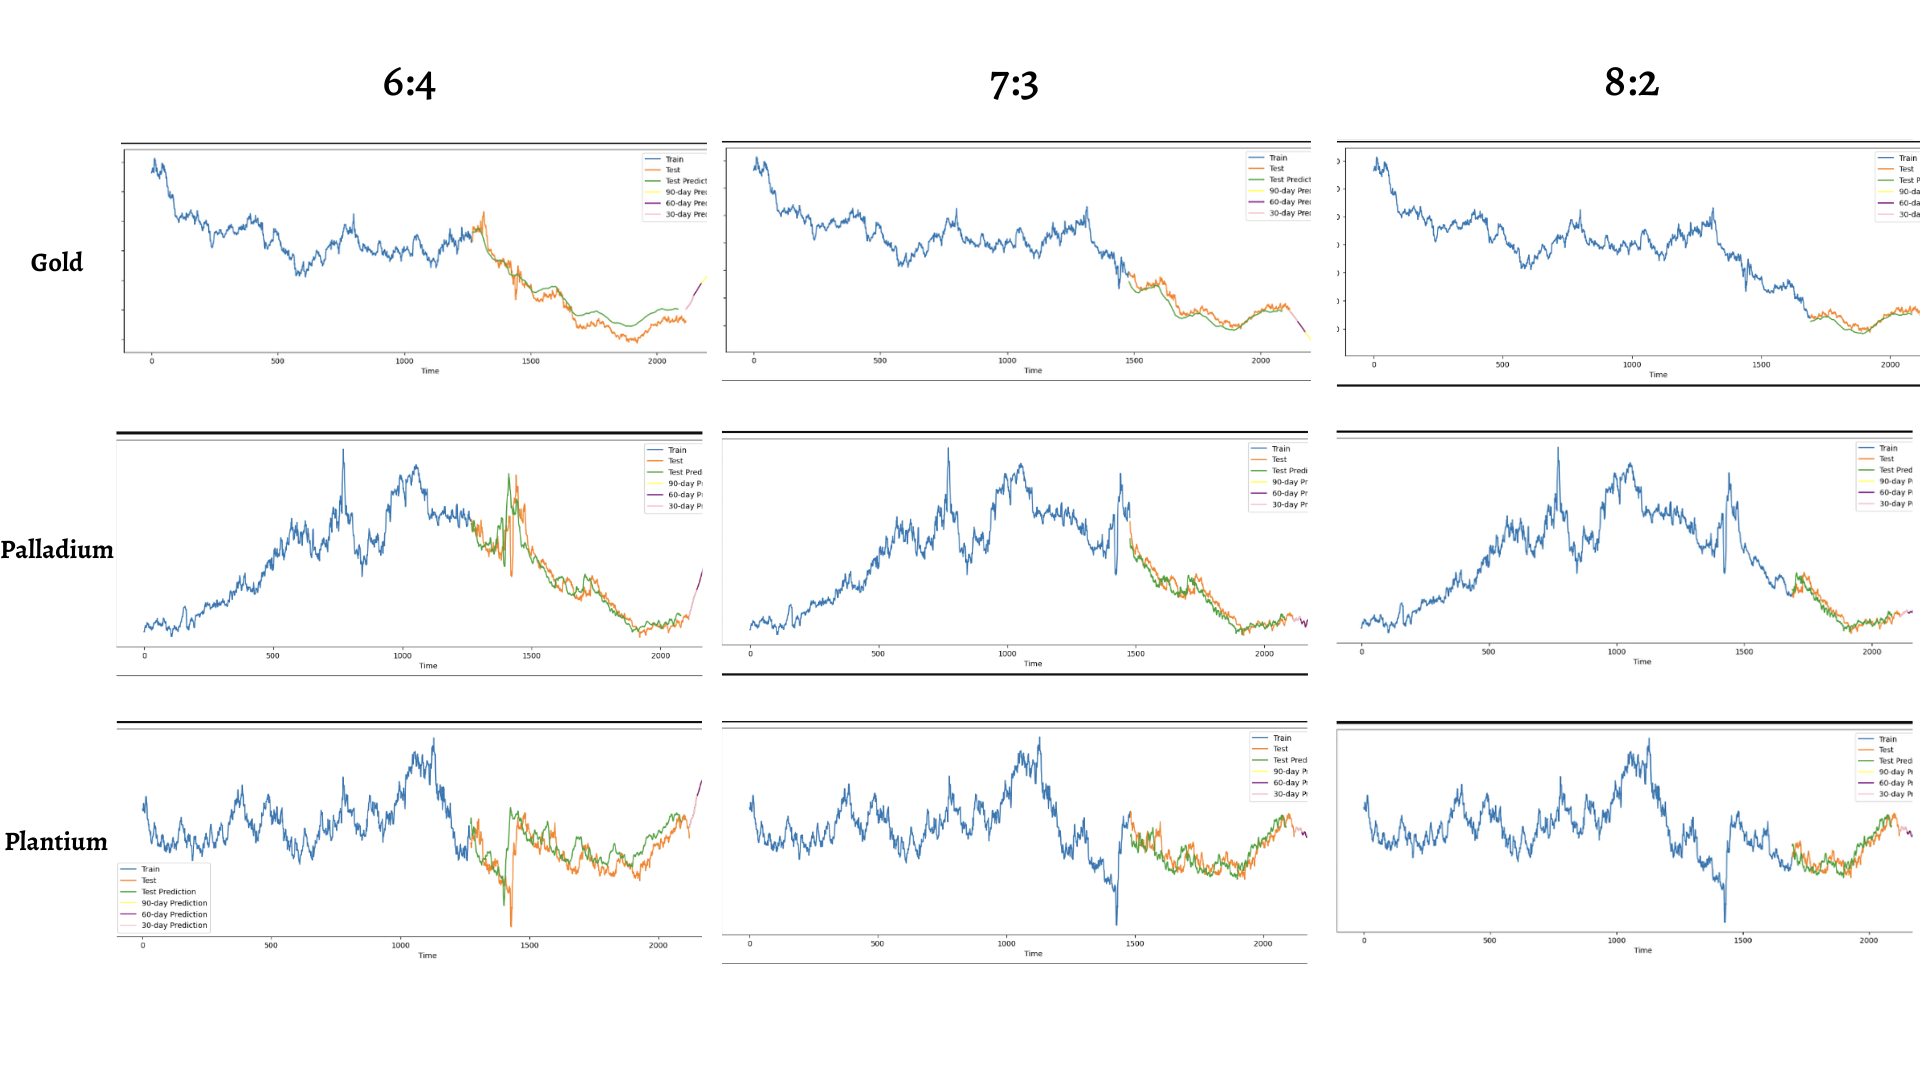
\includegraphics[width=0.45\textwidth]{img/SVR_result.png}}
\caption{Kết quả thực nghiệm SVR}
\label{fig}
\end{figure}

Madini O. Alassafi, Mutasem Jarrah, Reem Alotaibi\cite{10263962} đã sử dụng mô hình RNN và LSTM  để dự đoán sự lây lan của COVID-19 ở Malaysia, Morocco và Ả Rập Xê Út. Nghiên cứu cũng so sánh số ca mắc bệnh và số ca tử vong do COVID-19 ở Malaysia, Morocco và Ả Rập Xê Út. Sau đó, họ dự đoán số ca mắc và tử vong trong 7 ngày tiếp theo dựa trên dữ liệu có sẵn đến ngày 3 tháng 12 năm 2020. Kết quả độ chính xác của các mô hình lần lượt là 97.34\% RNN (Sigmoid), 93.32\% RNN (Tanh) và 99.27\% LSTM (ReLU). 

\begin{figure}[htbp]
\centerline{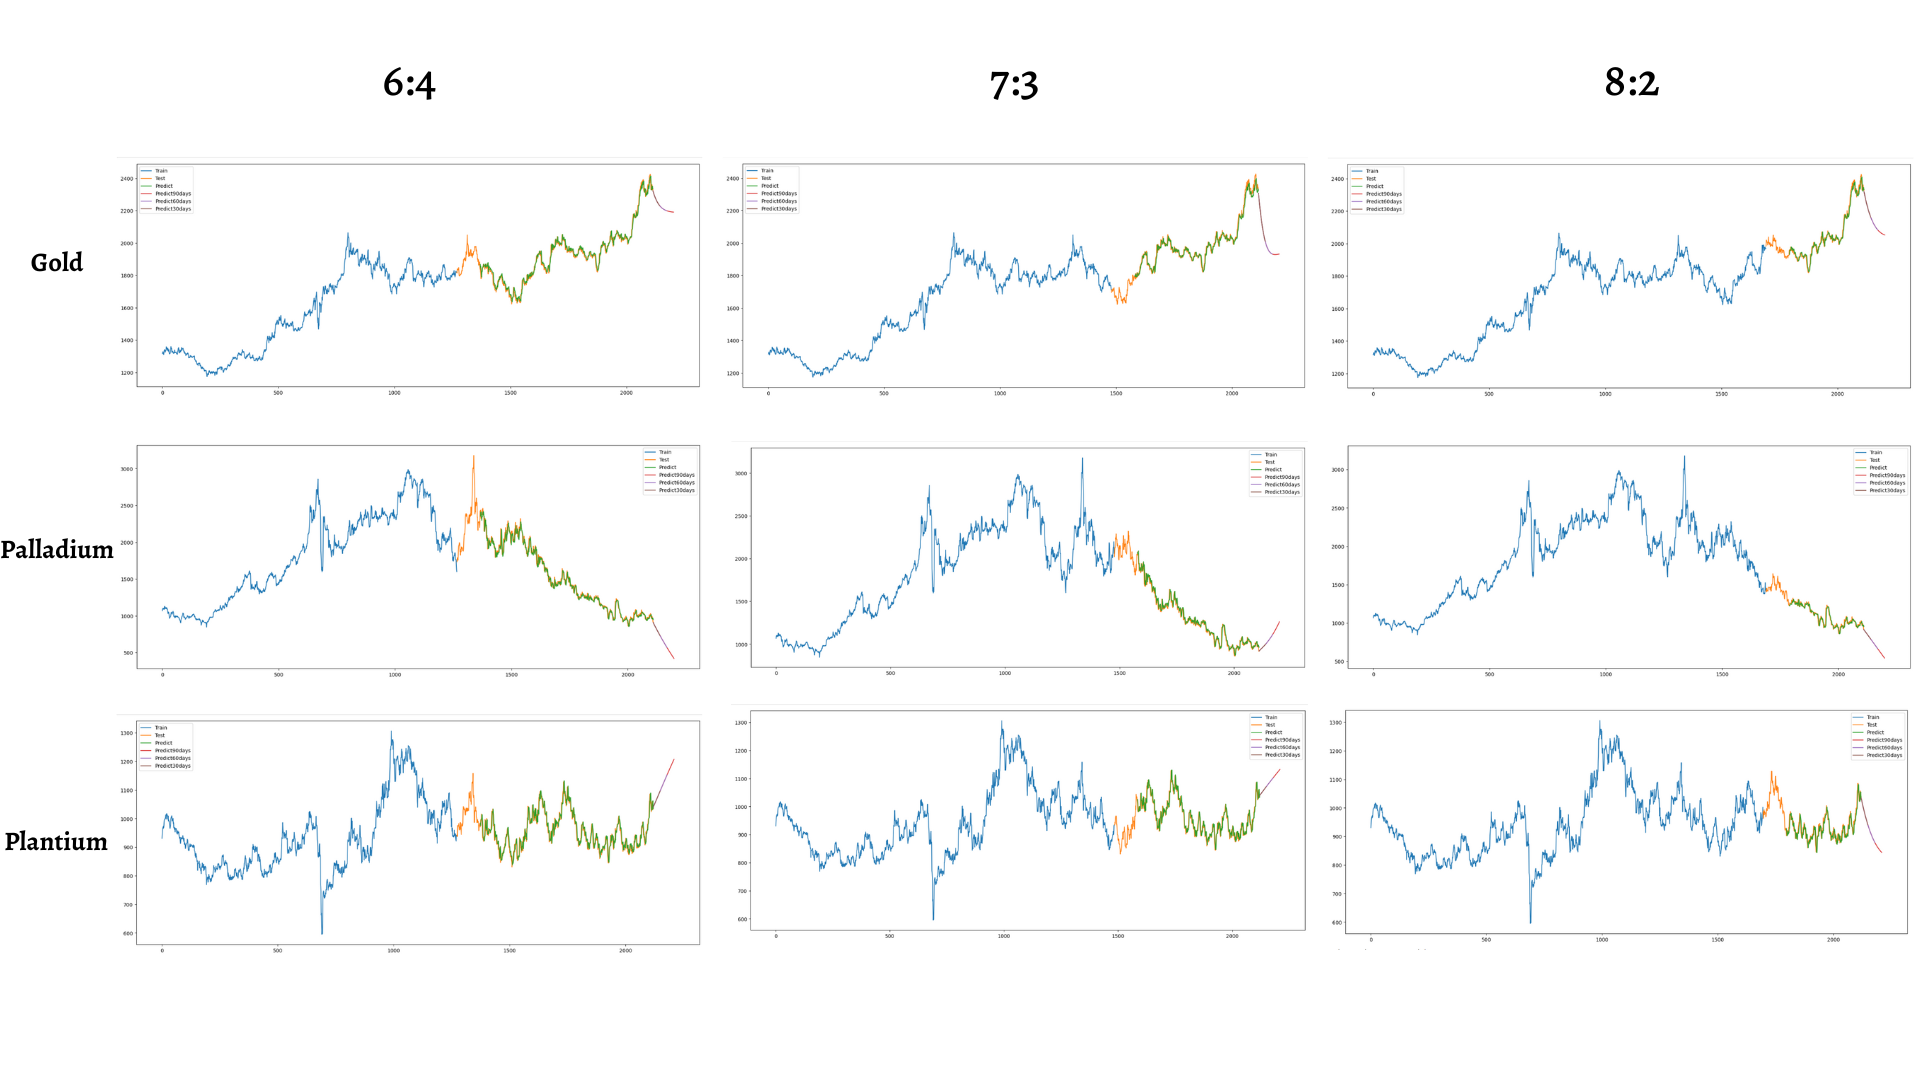
\includegraphics[width=0.5\textwidth]{img/GRU_result.png}}
\caption{Kết quả thực nghiệm GRU}
\label{fig}
\end{figure}

LSTM – là 1 dạng đặc biệt của mô hình RNN (Recurrent Neural Network), có khả năng học được các phụ thuộc. Phương pháp chính của mô hình LSTM là trạng thái tế bào (cell state), nó tương tự như 1 băng truyền chạy xuyên suốt tất cả các mắt xích và tương tác tuyến tính với các mắt xích đó vì vậy mà các thông tin dễ dàng truyền đi thông suốt mà không sợ bị thay đổi. LSTM sở hữu khả năng chọn lọc thông tin quan trọng bằng cách loại bỏ hoặc thêm vào trạng thái (state) của nó. Quá trình này được kiểm soát bởi các cấu trúc được gọi là cổng (gate). Mỗi cổng hoạt động như một bộ lọc thông tin, quyết định lượng thông tin được phép đi qua. Cụ thể, cổng bao gồm một lớp mạng sigmoid, tạo ra một giá trị trong khoảng từ 0 đến 1, đại diện cho tỷ lệ thông tin được truyền qua. Giá trị 0 nghĩa là không có thông tin nào được truyền qua, trong khi giá trị 1 cho phép tất cả thông tin đi qua. LSTM sử dụng ba cổng như vậy để quản lý và điều chỉnh trạng thái của tế bào: cổng quên (forget gate), cổng vào (input gate) và cổng ra (output gate).

\begin{figure}[htbp]
\centerline{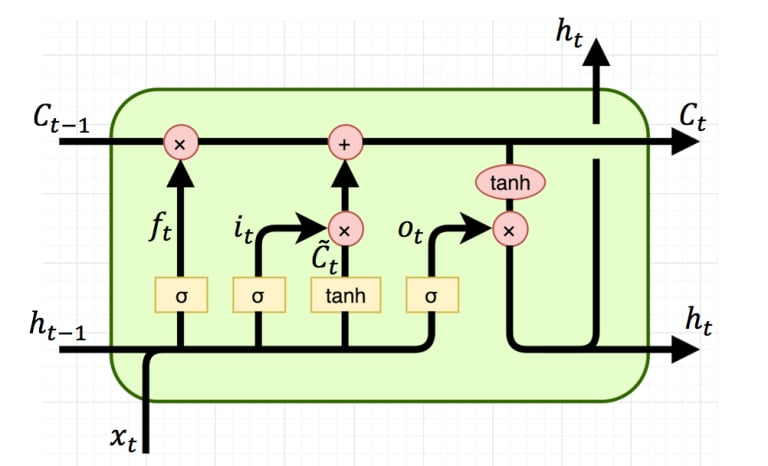
\includegraphics[width=0.4\textwidth]{img/LSTM.jpg}}
\caption{Kiến trúc LMST.}
\label{fig}
\end{figure}

Là phương pháp mô hình hóa biến thiên 2D theo thời gian để phân tích chuỗi thời gian tổng quát. Hành động tách các khoảng thời gian khác nhau khỏi chuỗi thời gian có thể làm giảm đáng kể độ phức tạp để xử lý các mô hình. Ngoài ra, FFT (Fast Fourier Transform) giúp nắm bắt được sự thay đổi trong và giữa các thời kỳ. Quá trình này cho phép chuỗi thời gian được tách rời có cách diễn giải vật lý rõ ràng hơn, nâng cao khả năng diễn giải của mô hình.

\begin{figure}[htbp]
\centerline{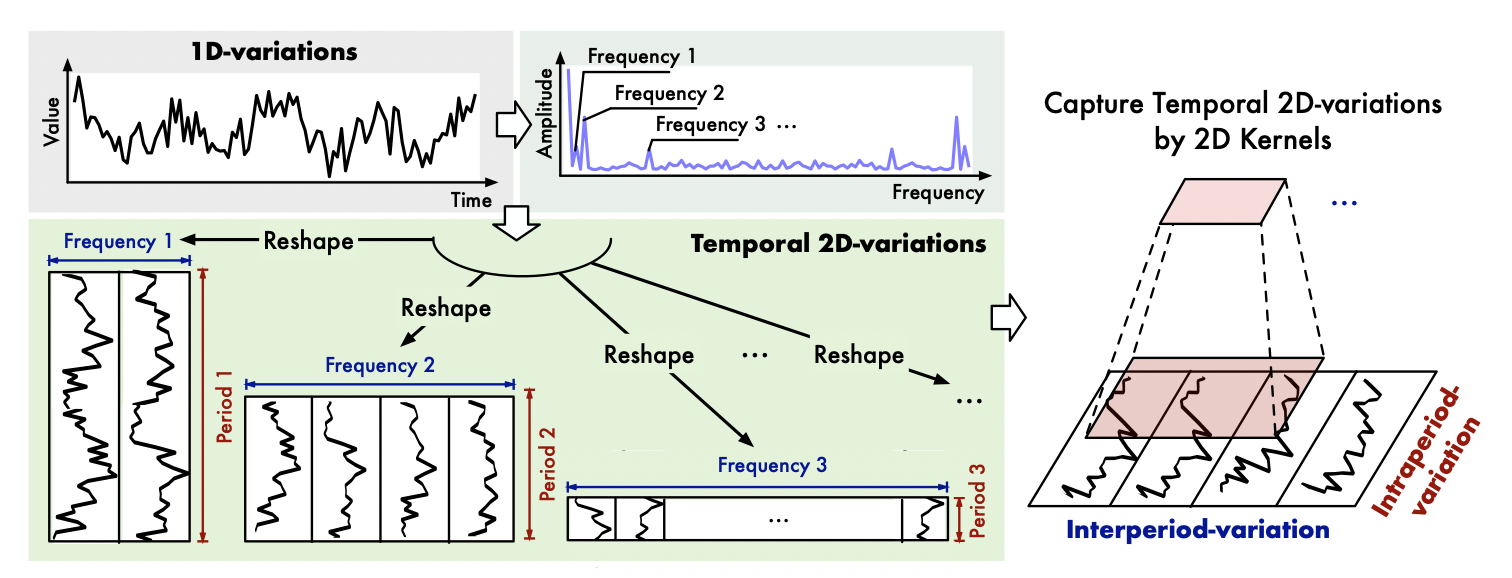
\includegraphics[width=0.4\textwidth]{img/2Dstructure.png}}
\caption{Minh họa cấu trúc 2D trong chuỗi thời gian.}
\label{fig}
\end{figure}

Bằng cách chuyển đổi dữ liệu chuỗi thời gian 1D thành một tập hợp các tensor 2D dựa trên nhiều chu kỳ, TimesNet phá vỡ giới hạn của chuỗi thời gian 1D và cho phép mô hình nắm bắt được sự biến đổi 2D theo thời gian của chuỗi thời gian.

\begin{figure}[htbp]
\centerline{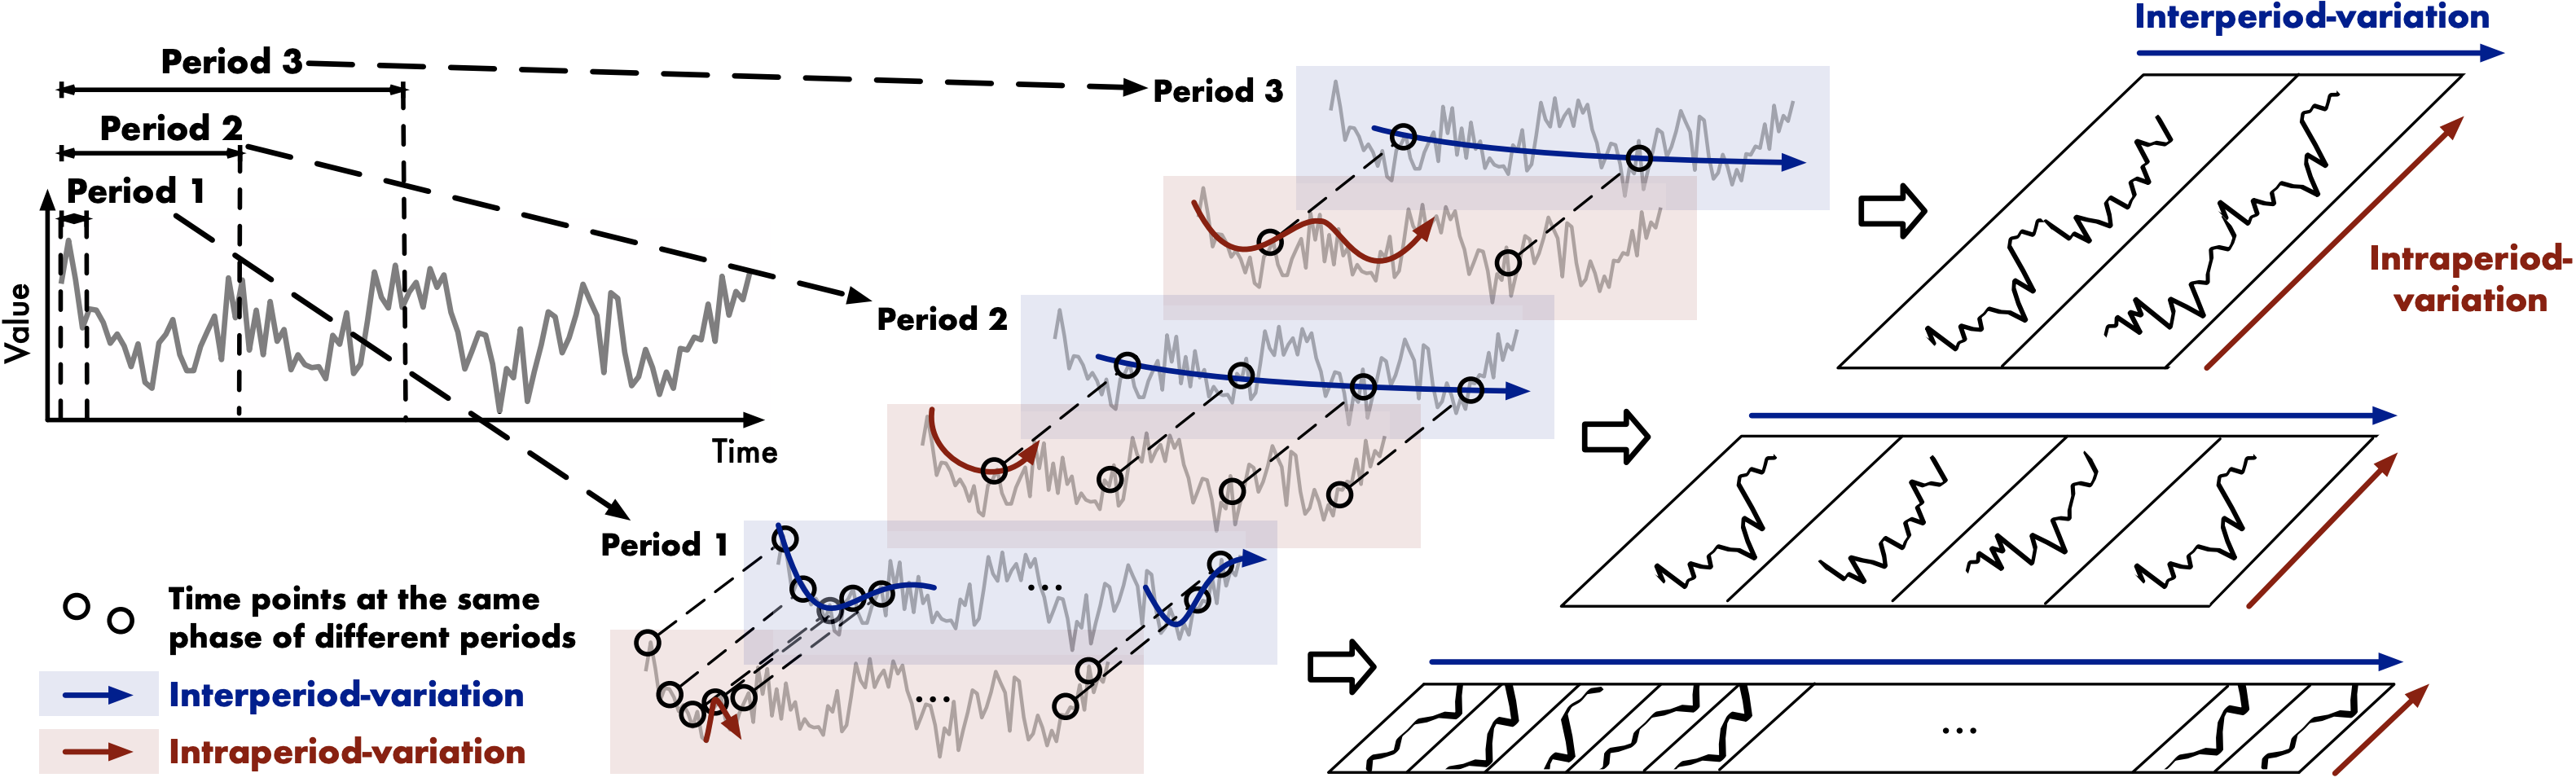
\includegraphics[width=0.4\textwidth]{img/2Dtensor.png}}
\caption{Chuyển đổi chuỗi thời gian 1D ban đầu thành một tập hợp các tensor 2D dựa trên nhiều chu kỳ.}
\label{fig}
\end{figure}

Autoformer: Phát triển từ Transformer, Autoformer như một kiến trúc phân rã mới với cơ chế Tự tương quan (Auto-corelation). Autoformer phá vỡ quy ước tiền xử lý về phân tách chuỗi và đổi mới nó thành khối bên trong cơ bản của các mô hình sâu. Thiết kế này trao quyền cho Autoformer khả năng phân rã lũy tiến cho chuỗi thời gian phức tạp. Hơn nữa, lấy cảm hứng từ lý thuyết quá trình ngẫu nhiên, mô hình này có cơ chế Tự tương quan dựa trên tính tuần hoàn của chuỗi, cơ chế này tiến hành khám phá phụ thuộc và tổng hợp biểu diễn ở cấp độ chuỗi phụ. Tự động tương quan vượt trội hơn khả năng tự chú ý cả về hiệu quả và độ chính xác. Trong dự báo dài hạn, Autoformer mang lại độ chính xác cao nhất, với mức cải thiện tương đối 38\% trên sáu điểm chuẩn, bao gồm năm ứng dụng thực tế: năng lượng, giao thông, kinh tế, thời tiết và bệnh tật.

\begin{table}[h!]
\centering
\tiny 
\setlength{\tabcolsep}{0.85pt} 
\begin{tabular}{|c|c|c|c|c|c|c|c|c|c|c|} 
\hline
\multirow{2}{*}{Mô hình} & \multirow{2}{*}{\makecell{Độ đo}} & \multicolumn{3}{c|}{Gold} & \multicolumn{3}{c|}{Platinum} & \multicolumn{3}{c|}{Palladium} \\ \cline{3-11}
& & 6:4 & 7:3 & 8:2 & 6:4 & 7:3 & 8:2 & 6:4 & 7:3 & 8:2 \\ \hline

\multirow{4}{*}{\makecell[c]{LR}} & MSE & 87892.376 & 60421.236 & 13670.77 & 33390.72 & 24896.165 & 13672.344 & 380725 & 288580 & 231493 \\
 &  & 76 & 236 & 7 & 2 & 65 & 44 & 5.595 & 8.893 & 0.054 \\ \cline{2-11}
 & RMSE & 296.466 & 245.807 & 116.922 & 182.731 & 157.785 & 116.929 & 1951.219 & 1698.767 & 1521.489 \\
 &  & 7 & 7 &  &  &  &  & 19 & 7 & 9 \\ \cline{2-11}
 & MAPE & 0.145 & 0.122 & 0.049 & 0.175 & 0.155 & 0.114 & 1.373 & 1.308 & 0.133 \\ \hline

\multirow{4}{*}{\makecell[c]{ETS}} & MSE & 16220.786 & 24542.912 & 36337.612 & 18391.562 & 16073.944 & 10671.415 & 70750.306 & 64441.255 & 7191.42 \\
 &  & 86 & 912 & 12 & 62 & 44 & 15 & 306 & 55 &  \\ \cline{2-11}
 & RMSE & 127.361 & 156.662 & 190.624 & 135.615 & 126.783 & 103.303 & 265.989 & 253.853 & 84.802 \\
 &  & 2 &  &  &  &  &  & 9 &  &  \\ \cline{2-11}
 & MAPE & 0.046 & 0.058 & 0.069 & 0.127 & 0.114 & 0.089 & 0.115 & 0.182 & 0.059 \\ \hline

 \multirow{4}{*}{\makecell[c]{ARIMA}} & MSE & 36441.460 & 46190.765 & 55921.673 & 9354.217 & 5213.863 & 4389.925 & 414476.127 & 352036.294 & 135397.298 \\
 &  &  &  &  &  &  &  &  &  &  \\ \cline{2-11}
 & RMSE & 190.896 & 214.920 & 236.477 & 96.717 & 72.207 & 66.256 & 643.798 & 593.326 & 367.963 \\
 &  &  &  &  &  &  &  &  &  &  \\ \cline{2-11}
 & MAPE & 0.069 & 0.082 & 0.088 & 0.090 & 0.053 & 0.047 & 0.430 & 0.441 & 0.299 \\ \hline

\multirow{4}{*}{\makecell[c]{RF}} & MSE & 13503.084 & 15563.667 & 22068.984 & 222.475 & 197.399 & 162.232 & 4506.977 & 4252.035 & 5670.472 \\
 &  &  &  &  &  &  &  &  &  &  \\ \cline{2-11}
 & RMSE & 116.202 & 124.754 & 148.556 & 14.915 & 14.049 & 12.737 & 67.134 & 65.207 & 75.302 \\
 &  &  &  &  &  &  &  &  &  &  \\ \cline{2-11}
 & MAPE & 0.026 & 0.029 & 0.038 & 0.011 & 0.010 & 0.010 & 0.032 & 0.037 & 0.046 \\ \hline

\multirow{4}{*}{\makecell[c]{SVM}} & MSE & 2923.408 & 1962.372 & 2093.366 & 893.129 & 794.283 & 714.362 & 21090.350 & 18557.479 & 24755.786 \\
 &  &  &  &  &  &  &  &  &  &  \\ \cline{2-11}
 & RMSE & 54.069 & 44.299 & 45.753 & 29.885 & 28.183 & 26.728 & 145.225 & 139.848 & 157.340 \\
 &  &  &  &  &  &  &  &  &  &  \\ \cline{2-11}
 & MAPE & 0.024 & 0.018 & 0.019 & 0.026 & 0.024 & 0.024 & 0.087 & 0.094 & 0.120 \\ \hline
 
\multirow{4}{*}{\makecell[c]{RNN}} & MSE & 499.596 & 515.097 & 1517.604 & 393.092 & 372.776 & 311.441 & 4196.248 & 1908.821 & 1879.004 \\
 &  &  &  &  &  &  &  &  &  &  \\ \cline{2-11}
 & RMSE & 22.352 & 22.696 & 39.956 & 19.827 & 19.307 & 17.648 & 64.779 & 43.690 & 43.348 \\
 &  &  &  &  &  &  &  &  &  &  \\ \cline{2-11}
 & MAPE & 0.009 & 0.009 & 0.013 & 0.016 & 0.015 & 0.014 & 0.027 & 0.024 & 0.031 \\ \hline

\multirow{4}{*}{\makecell[c]{GRU}} & MSE & 536.009 & 790.620 & 552.993 & 404.460 & 341.843 & 283.783 & 3888.186 & 1941.318 & 1134.122 \\
 &  &  &  &  &  &  &  &  &  &  \\ \cline{2-11}
 & RMSE & 23.151 & 28.117 & 23.515 & 20.111 & 18.488 & 16.845 & 62.355 & 44.060 & 33.676 \\
 &  &  &  &  &  &  &  &  &  &  \\ \cline{2-11}
 & MAPE & 0.008 & 0.010 & 0.008 & 0.015 & 0.014 & 0.013 & 0.025 & 0.023 & 0.021 \\ \hline
 
\multirow{4}{*}{\makecell[c]{LSTM}} & MSE & 1136.599 & 1457.405 & 560.276 & 539.192 & 300.794 & 316.181 & 4022.841 & 2125.158 & 1378.915 \\
 &  &  &  &  &  &  &  &  &  &  \\ \cline{2-11}
 & RMSE & 33.713 & 38.176 & 23.67 & 23.221 & 17.343 & 17.782 & 63.425 & 46.099 & 37.133 \\
 &  &  &  &  &  &  &  &  &  &  \\ \cline{2-11}
 & MAPE & 0.013 & 0.015 & 0.008 & 0.019 & 0.015 & 0.015 & 0.027 & 0.026 & 0.025 \\ \hline

\multirow{4}{*}{\makecell[c]{TimesNet}} & MSE & 496.222 & 350.124 & 372.906 & 333.390 & 252.735 & 193.083 & 3080.777 & 2100.171 & 888.844 \\
 &  &  &  &  &  &  &  &  &  &  \\ \cline{2-11}
 & RMSE & 22.276 & 18.711 & 19.310 & 18.258 & 15.897 & 13.895 & 55.504 & 45.827 & 29.813 \\
 &  &  &  &  &  &  &  &  &  &  \\ \cline{2-11}
 & MAPE & 0.008 & 0.006 & 0.007 & 0.015 & 0.013 & 0.011 & 0.022 & 0.025 & 0.019 \\ \hline
 
\multirow{4}{*}{\makecell[c]{Autoformer}} & MSE & 8768.156 & 7598.881 & 6137.704 & 3299.357 & 2104.744 & 1820.022 & 19418.751 & 10928.070 & 5629.101 \\
 &  &  &  &  &  &  &  &  &  &  \\ \cline{2-11}
 & RMSE & 93.638 & 87.171 & 78.343 & 57.440 & 45.877 & 42.661 & 139.351 & 104.537 & 75.027 \\
 &  &  &  &  &  &  &  &  &  &  \\ \cline{2-11}
 & MAPE & 0.036 & 0.030 & 0.024 & 0.046 & 0.037 & 0.035 & 0.061 & 0.056 & 0.050 \\ \hline

\end{tabular}
\label{table:my_table}
\end{table}

Bảng trên ghi nhận các giá trị độ đo MSE, RMSE, MAPE của các mô hình Linear Regression (LR), Exponential Smoothing Trend (ETS), ARIMA, Random Forest (RF), Support Vector Machine (SVM), Recurrent Neural Network (RNN), Gated Recurrent Unit  (GRU), Long Short Term Memory (LSTM), Timesnet, Autoformer trên tập test của ba bộ dữ liệu Gold, Platinum, Palladium theo 3 tỉ lệ train:test là: 6:4, 7:3, 8:2.

Các mô hình như RF và SVM thường cho kết quả tốt nhất với MSE và RMSE thấp, đặc biệt là với Palladium. Các mô hình deep learning như RNN, GRU, LSTM và các mô hình mạng nơ-ron TimesNet và Autoformer cũng cho thấy khả năng dự đoán tốt, đặc biệt là với các chỉ số MAPE thấp hơn so với các mô hình cơ bản như LR, ETS và ARIMA.

RF và SVM thường là lựa chọn ổn định cho việc dự đoán kim loại nhờ vào sự cân bằng giữa hiệu suất và ổn định. Các mô hình deep learning như Autoformer cũng cho thấy tiềm năng với các chỉ số đánh giá đứng đầu trong các thử nghiệm. Lựa chọn mô hình phụ thuộc vào các yếu tố như độ chính xác mong muốn và tính ổn định của kết quả dự đoán.

Dựa trên các thông tin từ bảng dữ liệu và các phân tích trên, lựa chọn mô hình phù hợp như RF, SVM hoặc Autoformer có thể giúp cải thiện dự đoán và đưa ra quyết định hiệu quả trong thị trường thực tế, đặc biệt là đối với các thị trường kim loại quý như Gold, Platinum và Palladium.


\section{Kết luận}
Trong bài báo này, chúng tôi đã thực hiện việc áp dụng các mô hình thống kê, học máy và học sâu để dự báo giá kim loại quý. Chúng tôi đã sử dụng các mô hình: Linear Regression (LR), Exponential Smoothing Trend (ETS), ARIMA, Random Forest (RF), Support Vector Regression (SVR), Recurrent Neural Network (RNN), Gated Recurrent Unit  (GRU), Long Short Term Memory (LSTM), Timesnet, Autoformer trên ba bộ dữ liệu khác nhau để dự báo giá kim loại quý. Qua đó, chúng tôi đánh giá và so sánh hiệu suất của từng mô hình cho thấy TimesNet, RNN và GRU có kết quả khá tốt. Điều này chỉ ra tiềm năng của các mô hình dựa trên mạng nơ-ron sâu trong lĩnh vực dự báo giá kim loại quý. 

Dù đạt được một số kết quả tích cực, nghiên cứu của chúng tôi cũng gặp phải một số thách thức. Một trong những thách thức đó là sự phức tạp và biến động của thị trường kinh tế, điều này làm cho việc dự báo giá kim loại trở nên khó khăn hơn.

Trong tương lai, chúng tôi dự định sẽ tiếp tục nghiên cứu và áp dụng các kỹ thuật tinh chỉnh mô hình để nâng cao hiệu quả dự báo. Ngoài ra, các mô hình nơ-ron sâu như TimesNet, RNN và GRU không chỉ giúp cải thiện độ chính xác của dự báo mà còn mở ra những cơ hội mới trong việc áp dụng trí tuệ nhân tạo để phân tích và dự báo các biến động phức tạp trong thị trường kim loại quý. Sự kết hợp giữa khả năng học hỏi sâu và khả năng xử lý dữ liệu chuỗi của các mạng nơ-ron này làm cho chúng trở thành công cụ quan trọng và hiệu quả trong nghiên cứu và thực tiễn đầu tư vàng (Gold), bạch kim (Platinum) và Palladium. Bên cạnh đó, chúng tôi sẽ xem xét việc sử dụng các mô hình mới nhất và phát triển phương pháp kết hợp giữa các mô hình khác nhau để tăng độ chính xác và độ tin cậy của dự báo. Chúng tôi cũng sẽ mở rộng phạm vi nghiên cứu bằng cách sử dụng thêm nhiều dữ liệu từ các thị trường kim loại quý khác nhau nhằm đạt được sự dự báo chính xác hơn.

\begin{center}
\textbf{ĐÓNG GÓP CỦA CÁC THÀNH VIÊN}
\end{center}
\textbf{Phan Minh Trí}: Kiểm tra – Chỉnh sửa, Kết luận, ARIMA, Random Forest.
\textbf{Trần Hạnh Thảo}: Đối tượng nghiên cứu, LR, ETS.
\textbf{Nguyễn Thị Tường Vi}: Tóm tắt nội dung, Độ đo, SVM, RNN.
\textbf{Lê Nguyễn Hoàng Huy}: Lời cảm ơn, GRU, TimesNet.
\textbf{Vương Thanh Linh}: Đặt vấn đề, LSTM, AutoFormer.

\begin{center}
\textbf{LỜI CẢM ƠN}
\end{center}

Nhóm xin chân thành cảm ơn PGS. TS. Nguyễn Đình Thuân và Kỹ sư Nguyễn Minh Nhựt vì sự hướng dẫn và đóng góp quý báu trong quá trình thực hiện bài báo này. Sự chỉ dẫn chuyên môn và kiến thức sâu rộng của PGS. TS. Nguyễn Đình Thuân cùng với sự hỗ trợ tận tình từ Kỹ sư Nguyễn Minh Nhựt đã cung cấp cho nhóm những nền tảng lý thuyết và phương pháp nghiên cứu cần thiết, giúp nhóm hiểu rõ hơn về kỹ thuật phân tích chuỗi thời gian và áp dụng vào dự báo giá kim loại quý.

Nhóm cũng xin bày tỏ lòng biết ơn đến các thành viên. Sự hợp tác, hỗ trợ lẫn nhau và chia sẻ kiến thức trong nhóm đã tạo nên một môi trường làm việc tích cực và là động lực để vượt qua những thách thức trong quá trình nghiên cứu. Những ý kiến đóng góp và các cuộc thảo luận nhóm đã giúp nhóm mở rộng tầm nhìn và hoàn thiện nội dung của bài báo.

Cuối cùng, nhóm xin gửi lời cảm ơn tới tất cả những ai đã đóng góp và hỗ trợ nhóm trong quá trình này. Sự đóng góp và hỗ trợ này đã đóng vai trò quan trọng trong việc hoàn thành bài báo và mang lại giá trị cho lĩnh vực nghiên cứu dự đoán. Nhóm hy vọng rằng công trình này sẽ được phổ biến rộng rãi và tiếp tục khám phá những tiềm năng và ứng dụng mới trong lĩnh vực này.

\printbibliography
\end{document}
